\documentclass[11pt]{article}
%%%%%%%%%%%%%%%%%%%%%%%%%%%%%%%%%%%%%%%%%%%%%%%%%%%%%%%%%%%%%%%
% DO NOT EDIT THIS FILE UNLESS YOU KNOW WHAT YOU ARE DOING!!! %
%%%%%%%%%%%%%%%%%%%%%%%%%%%%%%%%%%%%%%%%%%%%%%%%%%%%%%%%%%%%%%%

\usepackage[]{authblk}
\usepackage{graphicx}
\usepackage{color}
\usepackage{longtable}
\usepackage{hanging}
\usepackage{indentfirst}
\usepackage{setspace}
\usepackage{enumitem}
\usepackage{verbatim}
\usepackage{upgreek}
\usepackage{framed}
\usepackage{ textcomp }
\usepackage{url}
\usepackage{soul}
\usepackage{amsmath, amsfonts,amssymb,mathrsfs}
\usepackage{fancyhdr}
\usepackage[compact]{titlesec}
\usepackage[T1]{fontenc}
\usepackage{lmodern}
\usepackage[utf8]{inputenc}
\usepackage[export]{adjustbox}

\usepackage[backend=bibtex,hyperref=true,citestyle=authoryear,bibstyle=authortitle,firstinits=true,terseinits=true,doi=false,url=false,eprint=false,maxbibnames=10,maxcitenames=2]{biblatex}
\input{biblatex_macros}

\setlist{nolistsep}

\setlength{\evensidemargin}{0in}
\setlength{\headheight}{0in}
\setlength{\headsep}{0in}
\setlength{\oddsidemargin}{-0.25in}
\setlength{\paperheight}{11in}
\setlength{\paperwidth}{8.5in}
\setlength{\tabcolsep}{0in}
\setlength{\textheight}{9in}
\setlength{\textwidth}{7in}
\setlength{\topmargin}{0in}
\setlength{\topskip}{0in}
\setlength{\voffset}{0in}
\parskip = 0.15in
\pagestyle{plain}
\setlength{\parindent}{0cm}

\definecolor{citescol}{RGB}{194,101,1}
\definecolor{urlscol}{RGB}{0,150,206}
\definecolor{linkscol}{RGB}{149,0,207}
\definecolor{mycol}{RGB}{25,23,191}
\definecolor{outputcol}{RGB}{34,139,34}
\definecolor{tcol}{RGB}{165,0,14}


\DeclareMathAlphabet{\msfsl}{T1}{cmr}{m}{it}
\DeclareMathAlphabet{\msyf}{OMX}{pcr}{m}{it}
\newcommand{\alf}{\upalpha}
\newcommand{\hilight}[1]{\colorbox{yellow}{#1}}

\newcommand{\levelone}[1]{
\bigskip
\noindent{\LARGE{\textsc{#1}}}
\vspace {0.05in}
}

\newcommand{\leveltwo}[1]{
\bigskip
\noindent{\Large{\textit{#1}}}
\vspace {-1mm}
}

\newcommand{\descriptionhead}[1]{
\noindent{\textcolor{mycol}{\textbf{\textit{#1}}}}\\ \vspace{-7mm}
}

\newcommand{\dhead}[1]{
\noindent{\textbf{\textit{#1 --}}}
}



\newcommand{\exs}[1]{
\vspace{-4mm}
\begin{itemize}
\item #1 \\ \vspace{-8mm}
\end{itemize}
}

\newcommand{\nbo}[1]{{\color{red}{#1}}}


\newcommand{\stepbullet}{\noindent \textbullet \ }
\newcommand{\mi}[1]{\textbf{\textit{#1}}}


\newcommand{\levelthree}[1]{\textit{#1 --}}


%\bibliographystyle{apalike}
%\bibpunct[; ]{(}{)}{;}{a}{,}{;}


\usepackage[breaklinks]{hyperref}
\usepackage[all]{hypcap}
\hypersetup{colorlinks=true,linkcolor=linkscol,citecolor=citescol,urlcolor=urlscol}


\newcommand{\R}{\texttt{R} }
\newcommand{\TESS}{\texttt{TESS}}
\newcommand{\PBD}{\texttt{PBD}}
\newcommand{\DDD}{\texttt{DDD}}
\newcommand{\Laser}{\texttt{laser}}
\newcommand{\TreePar}{\texttt{TreePar}}
\newcommand{\diversitree}{\texttt{diversitree}}
\newcommand{\RevBayes}{\texttt{RevBayes}}
\newcommand{\Rev}{\texttt{Rev}}
\newcommand{\MrBayes}{\texttt{MrBayes}}
\newcommand{\BEAST}{\texttt{BEAST}}
\newcommand{\PhyloBayes}{\texttt{PhyloBayes}}
\newcommand{\PAML}{\texttt{PAML}}

\let\otheriint\iint
\let\iint\relax
\usepackage{ wasysym }

\usepackage{framed}
\usepackage[]{listings}
%\usepackage{fontspec}
\usepackage{placeins}
\usepackage{epstopdf}



\lstset{backgroundcolor=\color[rgb]{0.972,0.972,0.972},
		tabsize=4,
		rulecolor=,
        basicstyle=\scriptsize,
        upquote=true,
        aboveskip={1.5\baselineskip},
        columns=fixed,
        showstringspaces=false,
        extendedchars=true,
        breaklines=true,
        prebreak = \raisebox{0ex}[0ex][0ex]{\ensuremath{\hookleftarrow}},
        frame=single,
        showtabs=false,
        showspaces=false,
        showstringspaces=false,
        identifierstyle=\ttfamily,
        keywordstyle=\color[rgb]{0,0,1},
        commentstyle=\color[rgb]{0.133,0.545,0.133},
        stringstyle=\color[rgb]{0.627,0.126,0.941}
}

\definecolor{shadecolor}{RGB}{194,225,255}

\setlength{\tabcolsep}{5pt}
\setlength{\topmargin}{-0.4in}
\setlength{\headheight}{14.5pt}
\pagestyle{fancy}

\newcommand{\taha}[1]{{\textcolor{red}{[TAH comment: #1]}}} % TAH comment

\titlespacing{\section}{0pt}{*0}{*0}
\titlespacing{\subsection}{0pt}{*0}{*0}
\titlespacing{\subsubsection}{0pt}{*0}{*0}

\titleformat{\section}
  {\normalfont\Large\bfseries\color{mycol}}
  {\thesection}{1em}{}

\titleformat{\subsection}
  {\normalfont\large\bfseries\color{mycol}}
  {\thesubsection}{1em}{}

\titleformat{\subsubsection}
  {\normalfont\bfseries\color{mycol}}
  {\thesubsubsection}{1em}{}

% command for MrBayes command-line step
\newcommand{\cl}[1]{{\texttt{\textbf{#1}}}}

\newcommand{\colx}[1]{{\textcolor{tcol}{#1}}}

\newcommand{\mbcl}[1]{\exs{\cl{MrBayes > {#1}}}}

\newcommand{\rbprmt}{RevBayes > } 
\newcommand{\rbcl}[1]{\exs{\cl{\rbprmt{#1}}}}
\newcommand{\rbout}[1]{\exs{\cl{\textcolor{outputcol}{#1}}}}
\newcommand{\rbdn}{{\Large \symbol{126}}} % This makes a copy/pasteable tilde
\newcommand{\rbclml}[1]{\exs{\cl{\ \ \ \ \ \ \ \ \ \ \ {#1}}}}

% text box settings
% requires compiling w/ XeLaTeX
%\newfontfamily\listingsfont[Scale=1.0]{Courier New}
%\lstset{basicstyle=\listingsfont, columns=texcl}
%\defaultfontfeatures{Mapping=tex-text}


\makeatletter
\lst@CCPutMacro\lst@ProcessOther {"2D}{\lst@ttfamily{-{}}{-{}}}
\@empty\z@\@empty
\makeatother


\usepackage{tikz}

\setlength{\topmargin}{-0.4in}
\setlength{\headheight}{14.5pt}
\pagestyle{fancy}

\usepackage[breaklinks]{hyperref}
\usepackage[all]{hypcap}
\hypersetup{colorlinks=true,linkcolor=linkscol,citecolor=citescol,urlcolor=urlscol}

\definecolor{lg}{gray}{0.75}
\def\gcirc{{%
    \setbox0\hbox{$\fullmoon$}%
    \rlap{\hbox to \wd0{\hss{$\textcolor{lg}{\newmoon}$}\hss}}\box0
}}



% Add your bibtex library here
\addbibresource{master_refs.bib}

%%%%%%%%%%%%%% Fixme setup
\definecolor{red}{HTML}{C92D39}

% syntax: \fixme{What needs to be fixed}
\newcommand{\fixme}[1]{\textcolor{red}{\texttt{{\bf FIX ME:} #1}}}
% Hide all fixmes by switching the line above to this:
%\newcommand{\fixme}[1]{}


\begin{document}
\renewcommand{\headrulewidth}{0.5pt}
\headsep = 20pt
\lhead{ }
\rhead{\textsc {BEAST v2 Tutorial}}

\thispagestyle{plain}

\begin{center}
\textbf{\LARGE Tutorial using BEAST v2.4.2}\\\vspace{2mm}
\textbf{\textcolor{mycol}{\Large Skyline Plots}}\\
\vspace{4mm}
{\Large {\em Nicola F. M\"uller and Louis du Plessis}}
\end{center}


Inference of past population dynamics using Bayesian Coalescent Skyline and Birth-Death Skyline plots.

\bigskip
\section{Background}

Population dynamics influence the shape of the tree and consequently, the shape of the tree contains some information about past population dynamics. The so-called Skyline methods allow to extract this information from phylogenetic trees in a non-parametric manner. It is non-parametric since there is no underlying system of differential equations governing the inference of these dynamics. In this tutorial we will look at two different methods to infer these dynamics from sequence data. The first one is the Bayesian Coalescent Skyline plot \citep{Drummond2005}, which is based on the coalescent model, and the second one is the Birth-Death skyline \citep{Stadler2013} plot based on the birth-death model. The conceptual difference between coalescent and birth-death approaches lies in the direction of the flow of time. In the coalescent, the time is modeled to go backwards, from present to past, while in the birth-death approach it is modeled to go forwards. Two other fundamental differences are the parameters that are inferred and the way sampling is treated. 


%\clearpage
%\newpage
\bigskip
\section{Programs used in this Exercise}\label{programsSec}

\descriptionhead{BEAST -- Bayesian Evolutionary Analysis Sampling Trees}

BEAST version 2.4.2 \citep{Bouckaert2014}. 

\descriptionhead{BEAUti -- Bayesian Evolutionary Analysis Utility}

GUI to create *.xml for BEAST.

\descriptionhead{Tracer} 

\href{http://tree.bio.ed.ac.uk/software/tracer}{Tracer} is a graphical tool for visualization and diagnostics of MCMC output, which summarizes the posterior estimates of various parameters sampled by the Markov Chain. It can be used for visual inspection and assessment of convergence of MCMC runs. It helps to quickly view median estimates and the 95\% highest posterior density intervals of the parameters, and calculates the effective sample sizes (ESS) of parameters. It also allows one to visualize possible parameter correlations.

\descriptionhead{R} 

We will be using \href{https://www.r-project.org}{R} to analyze the output of the birth-death skyline plot. We will start the provided R script from the terminal, hence there is no need for applications like RStudio which provides a graphical user interface for R. If you prefer using RStudio feel free to do so.

\newpage
\section{Practical: Bayesian and birth-death skyline plot}

In this tutorial we will estimate the dynamics of the Egyptian Hepatitis C epidemic from genetic sequence data collected in 1993.

The aim of this tutorial is to:
\begin{itemize}
\item learn how to infer population dynamics;
\item get to know how to choose the set-up of a skyline analysis;
\item get to know the advantages and disadvantages of the Bayesian Coalescent Skyline and the Birth-Death Skyline.
\end{itemize}

\bigskip
\subsection{The Data}
The dataset consists of an alignment of 63 Hepatitis C sequences sampled in 1993 in Egypt \citep{Ray2000}. This dataset has been used previously to test the performance of skyline methods \citep{Pybus2003,Drummond2005,Stadler2013}.

With an estimated $15-25\%$, Egypt has the highest Hepatits C prevalence in the world. In the mid 20$^{\mathrm{th}}$ century, the prevalence of Hepatitis C increased drastically (see Figure~\ref{fig:prevalence} for estimates). We will try to infer this increase from sequence data. 



%\fixme{maybe change later}
%The raw sequence data (*.nexus files), precooked runs, as well as an R script needed for run log analysis can be downloaded using the link below.


%\begin{framed}
%Download data, scripts and pre-cooked output files from:
%\begin{center}
%\href{google.com}{URL} 
%\end{center}
%\end{framed}
%\fixme{needs URL!}

\begin{figure}[h!]
\centering
\fbox{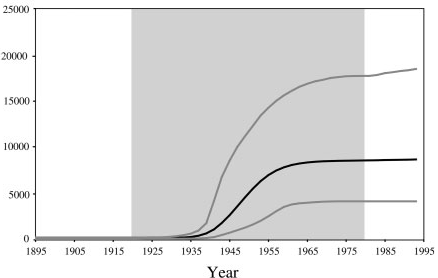
\includegraphics[scale=0.5]{figures/Estimated_number_hcv.png}}
\caption{\small The estimated number of Hepatitis C cases in Egypt~\citep{Pybus2003}.}
\label{fig:prevalence}
\end{figure}




\bigskip
\subsection{Creating the Analysis File with BEAUti}

We will use BEAUti to generate the configuration file for BEAST2 from the sequence alignment.

\bigskip
\subsubsection{Install BEAST 2 Plug-Ins}

While the Bayesian Coalescent Skyline plot is integrated in the core of BEAST2, we need to install the BDSKY package, which contains the birth-death skyline plot functionality. Installation of packages is done using the package manager, which is integrated into BEAUti. Open the package manager with \texttt{File > Manage Packages} in BEAUti. Select the BDSKY package and install it using the \texttt{Install/Upgrade} button (Figure~\ref{fig:install}).

%\begin{figure}[h!]
%\centering
%\fbox{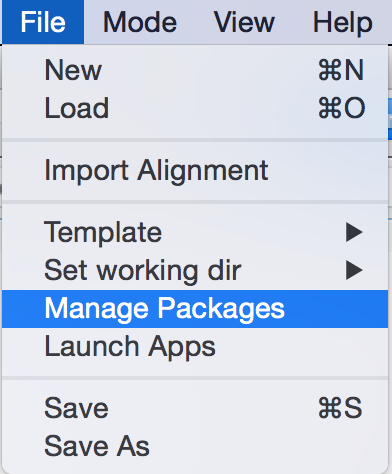
\includegraphics[width=0.2\textwidth]{figures/package_manager.png}}
%\caption{\small Open the package manager.}
%\label{fig:manager}
%\end{figure}
%\clearpage

\begin{figure}[h!]
\centering
\fbox{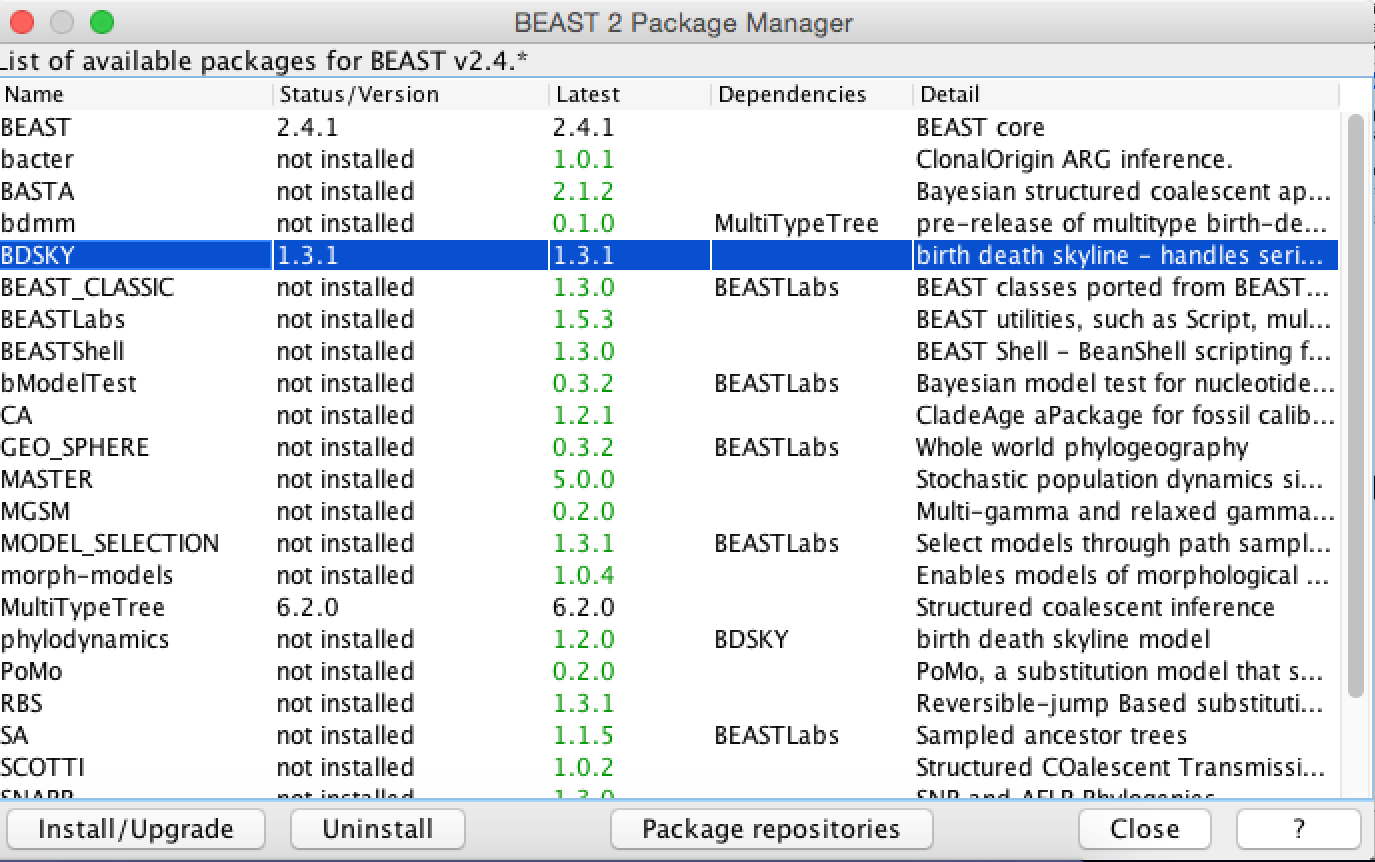
\includegraphics[scale=0.5]{figures/install_bdsky.png}}
\caption{\small Install the package BDSKY which contains the birth-death skyline functionality.}
\label{fig:install}
\end{figure}

\subsubsection{Setting up the analysis with Bayesian Coalescent Skyline}

To import the aligned sequences into BEAUti, use \texttt{File > Import Alignment} to select the *.nexus file.

%\begin{figure}[h!]
%\centering
%\fbox{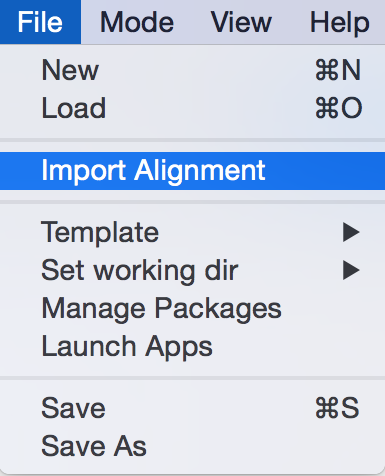
\includegraphics[width=0.2\textwidth]{figures/import_alignment.png}}
%\caption{\small import the alignment}
%\label{fig:import}
%\end{figure}

BEAUti will recognize the sequences from the \texttt{*.nexus} file as nucleotide data. It will do so for sequence files with the character set of \textbf{ATGC}. As soon as some positions are unknown, which can e.g. be indicated by an \textbf{N}, BEAUti will not recognize the data as nucleotides anymore, unless the type of data is specified in the \texttt{*.nexus} file.

After we have loaded the sequences into BEAUti, we have to specify the evolutionary model. We will be using the very general GTR model (Figure~\ref{fig:model}), which estimates transition probabilities between individual nucleotides separately, meaning that transition probabilities between e.g. \textbf{A} and \textbf{T} will be inferred separately to the ones between \textbf{A} and \textbf{C}. Additionally, we should allow for rate heterogeneity among sites. We can do this by changing the Gamma Category Count to 4 (normally between 4 and 6).

%\fixme{is this what you want?}
%Leave all the model parameters on their default values for the GTR.

\begin{figure}[h!]
\centering
\fbox{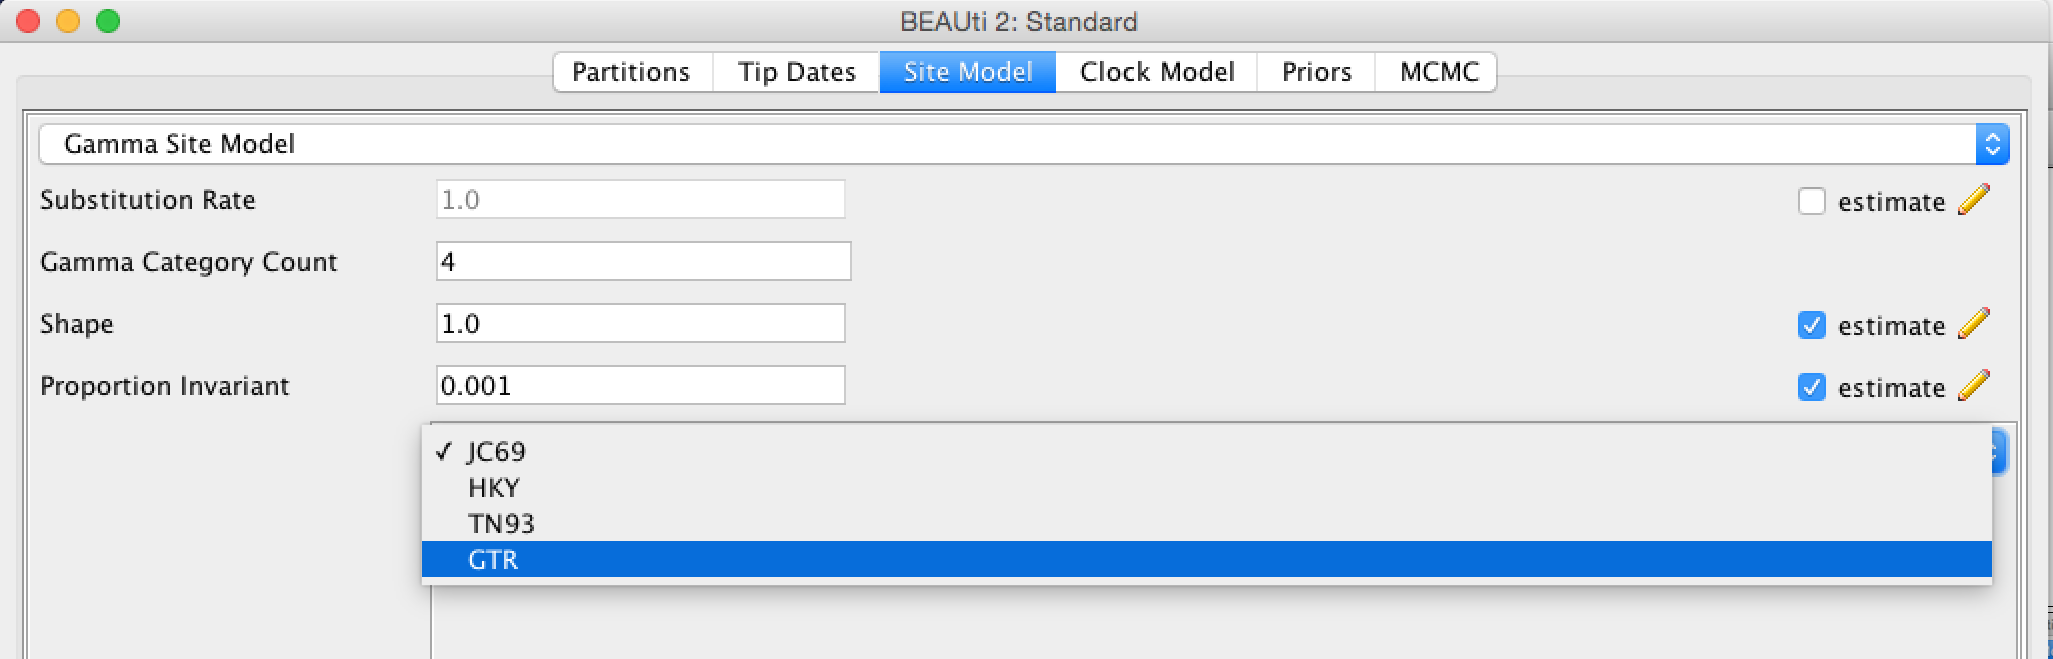
\includegraphics[width=\textwidth]{figures/choose_gtr.png}}
\caption{\small Set GTR as a site model. Also use a Gamma Category Count of 4}
\label{fig:model}
\end{figure}
\clearpage

As we use sequences that were sampled at the same point in time, we need to fix the clock rate\footnote{For more information on this please refer to the tutorial on molecular clocks}. We will use an estimate inferred in \citet{Pybus2001} to fix the clock rate. In this case all the samples were contemporaneous (at the same time) and the clock rate works as a mapping of the estimated tree branch lengths into calendar time.

We will keep the strict clock model and will set the \texttt{Clock.rate} to $0.00079$.

%as shown in Figure~\ref{fig:clockrate}.

%\begin{figure}[h!]
%\centering
%\fbox{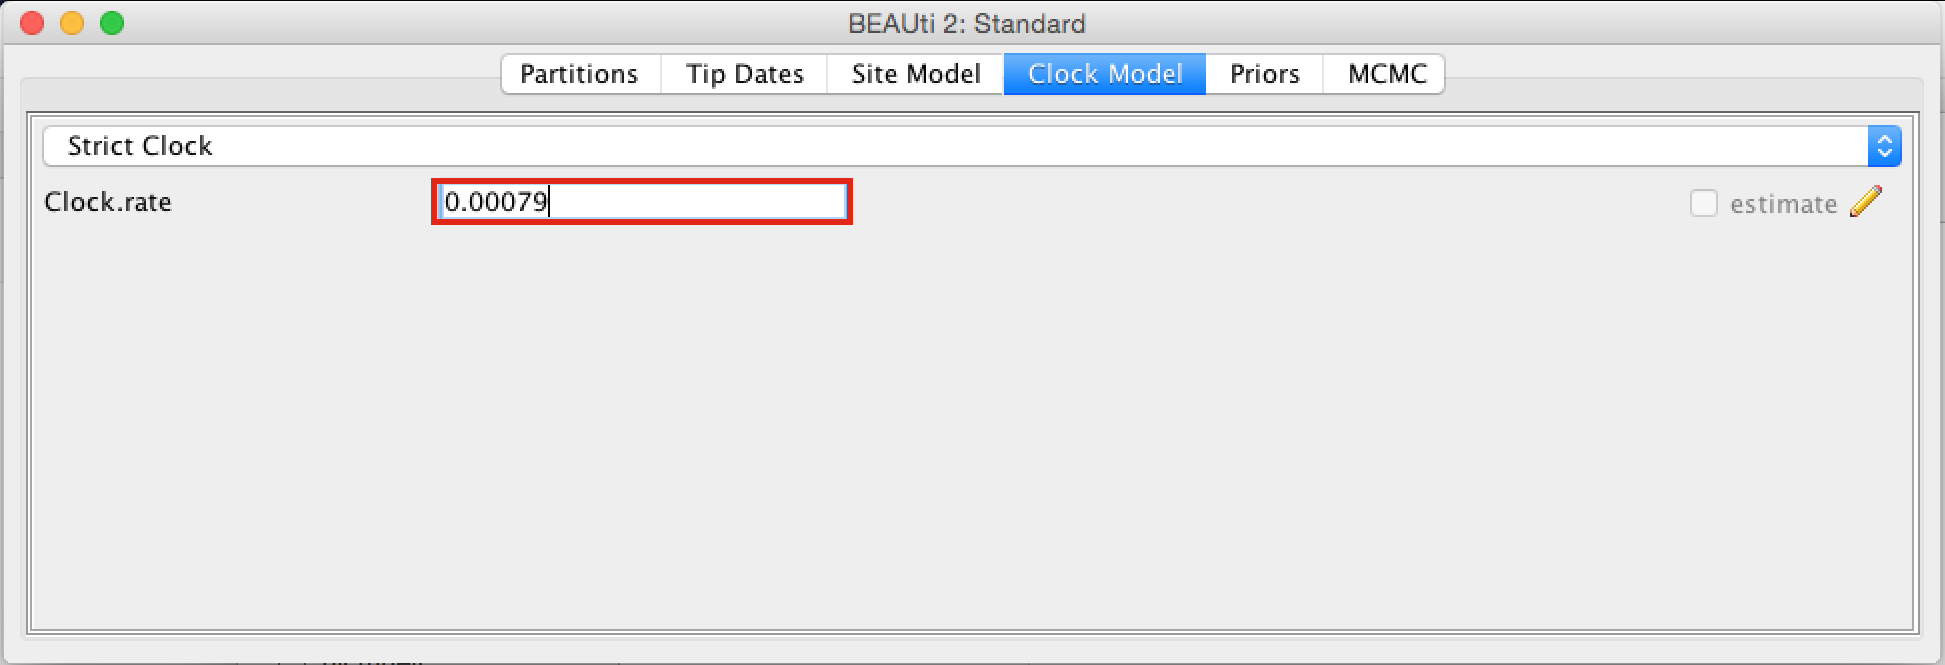
\includegraphics[width=\textwidth]{figures/set_clockrate.png}}
%\caption{\small Set the clock rate to $0.00079$.}
%\label{fig:clockrate}
%\end{figure}

Next, we need to go the the \texttt{Priors} tab and set the Bayesian Coalescent Skyline as a tree prior (Figure~\ref{fig:coalescent}).

\begin{figure}[h!]
\centering
\fbox{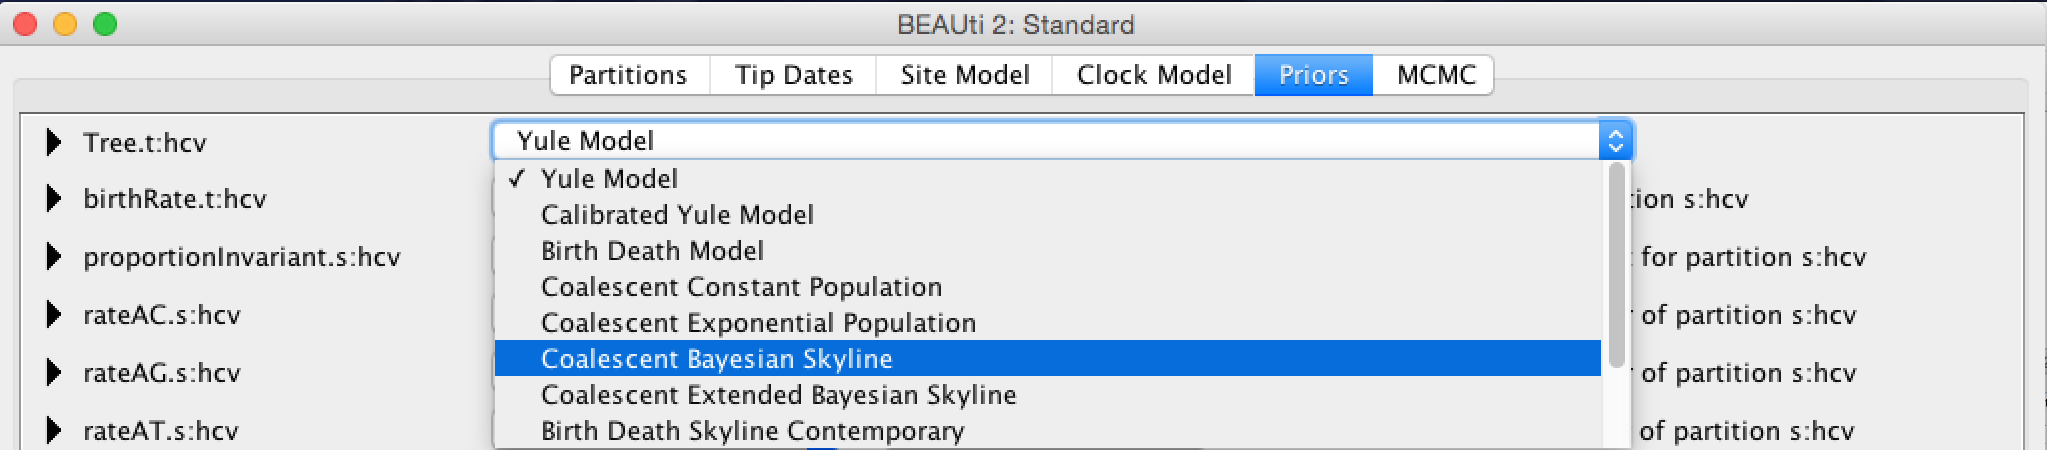
\includegraphics[width=\textwidth]{figures/choose_coalescentSkyline.png}}
\caption{\small Choose the Coalescent Bayesian Skyline as a population prior.}
\label{fig:coalescent}
\end{figure}

%\fixme{It has not been explained previously. Or do you mean that it should have been explained in class? Explain it once again here quickly anyway.}
The Bayesian Coalescent Skyline works by dividing the time between the present and the root of the tree into intervals, thus the number of these intervals has to be defined. Each interval will have a different effective population size. 
The Bayesian Coalescent Skyline will estimate the number of coalescent events within each interval (which is captured in the Group Size parameter) as well as the effective population size for that interval. The number of intervals is equal to the dimension specified. If we have $d$ intervals, the effective population size is allowed to change $d-1$ times. To specify the number of dimensions, we need to first go to the initialization panel. This is by default not visible \texttt{View > Show Initialization Panel}.

%\begin{figure}[h!]
%\centering
%\fbox{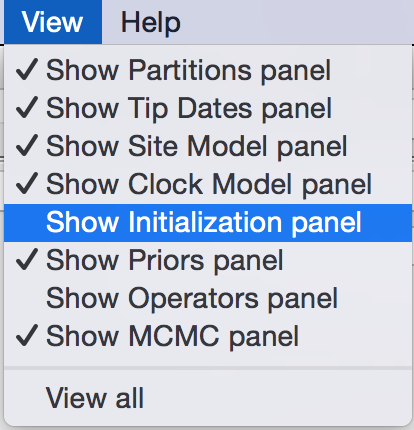
\includegraphics[width=0.2\textwidth]{figures/goto_initialization.png}}
%\caption{\small go to the initialization panel.}
%\label{fig:initialization}
%\end{figure}

%\fixme{This procedure needs to be explained better (what do you expand and what do you write where) as we didn't do this before. Also, 5 is the default value, you need to say it.}

For this analysis we will set the number of dimensions to $4$ (the default value is 5). Keep in mind that one has to change the dimension of \textbf{bPopSizes} as well as \textbf{bGroupSizes}. The dimension of both parameters has to be the same (Figure~\ref{fig:dimensions}).

\begin{figure}[h!]
\centering
\fbox{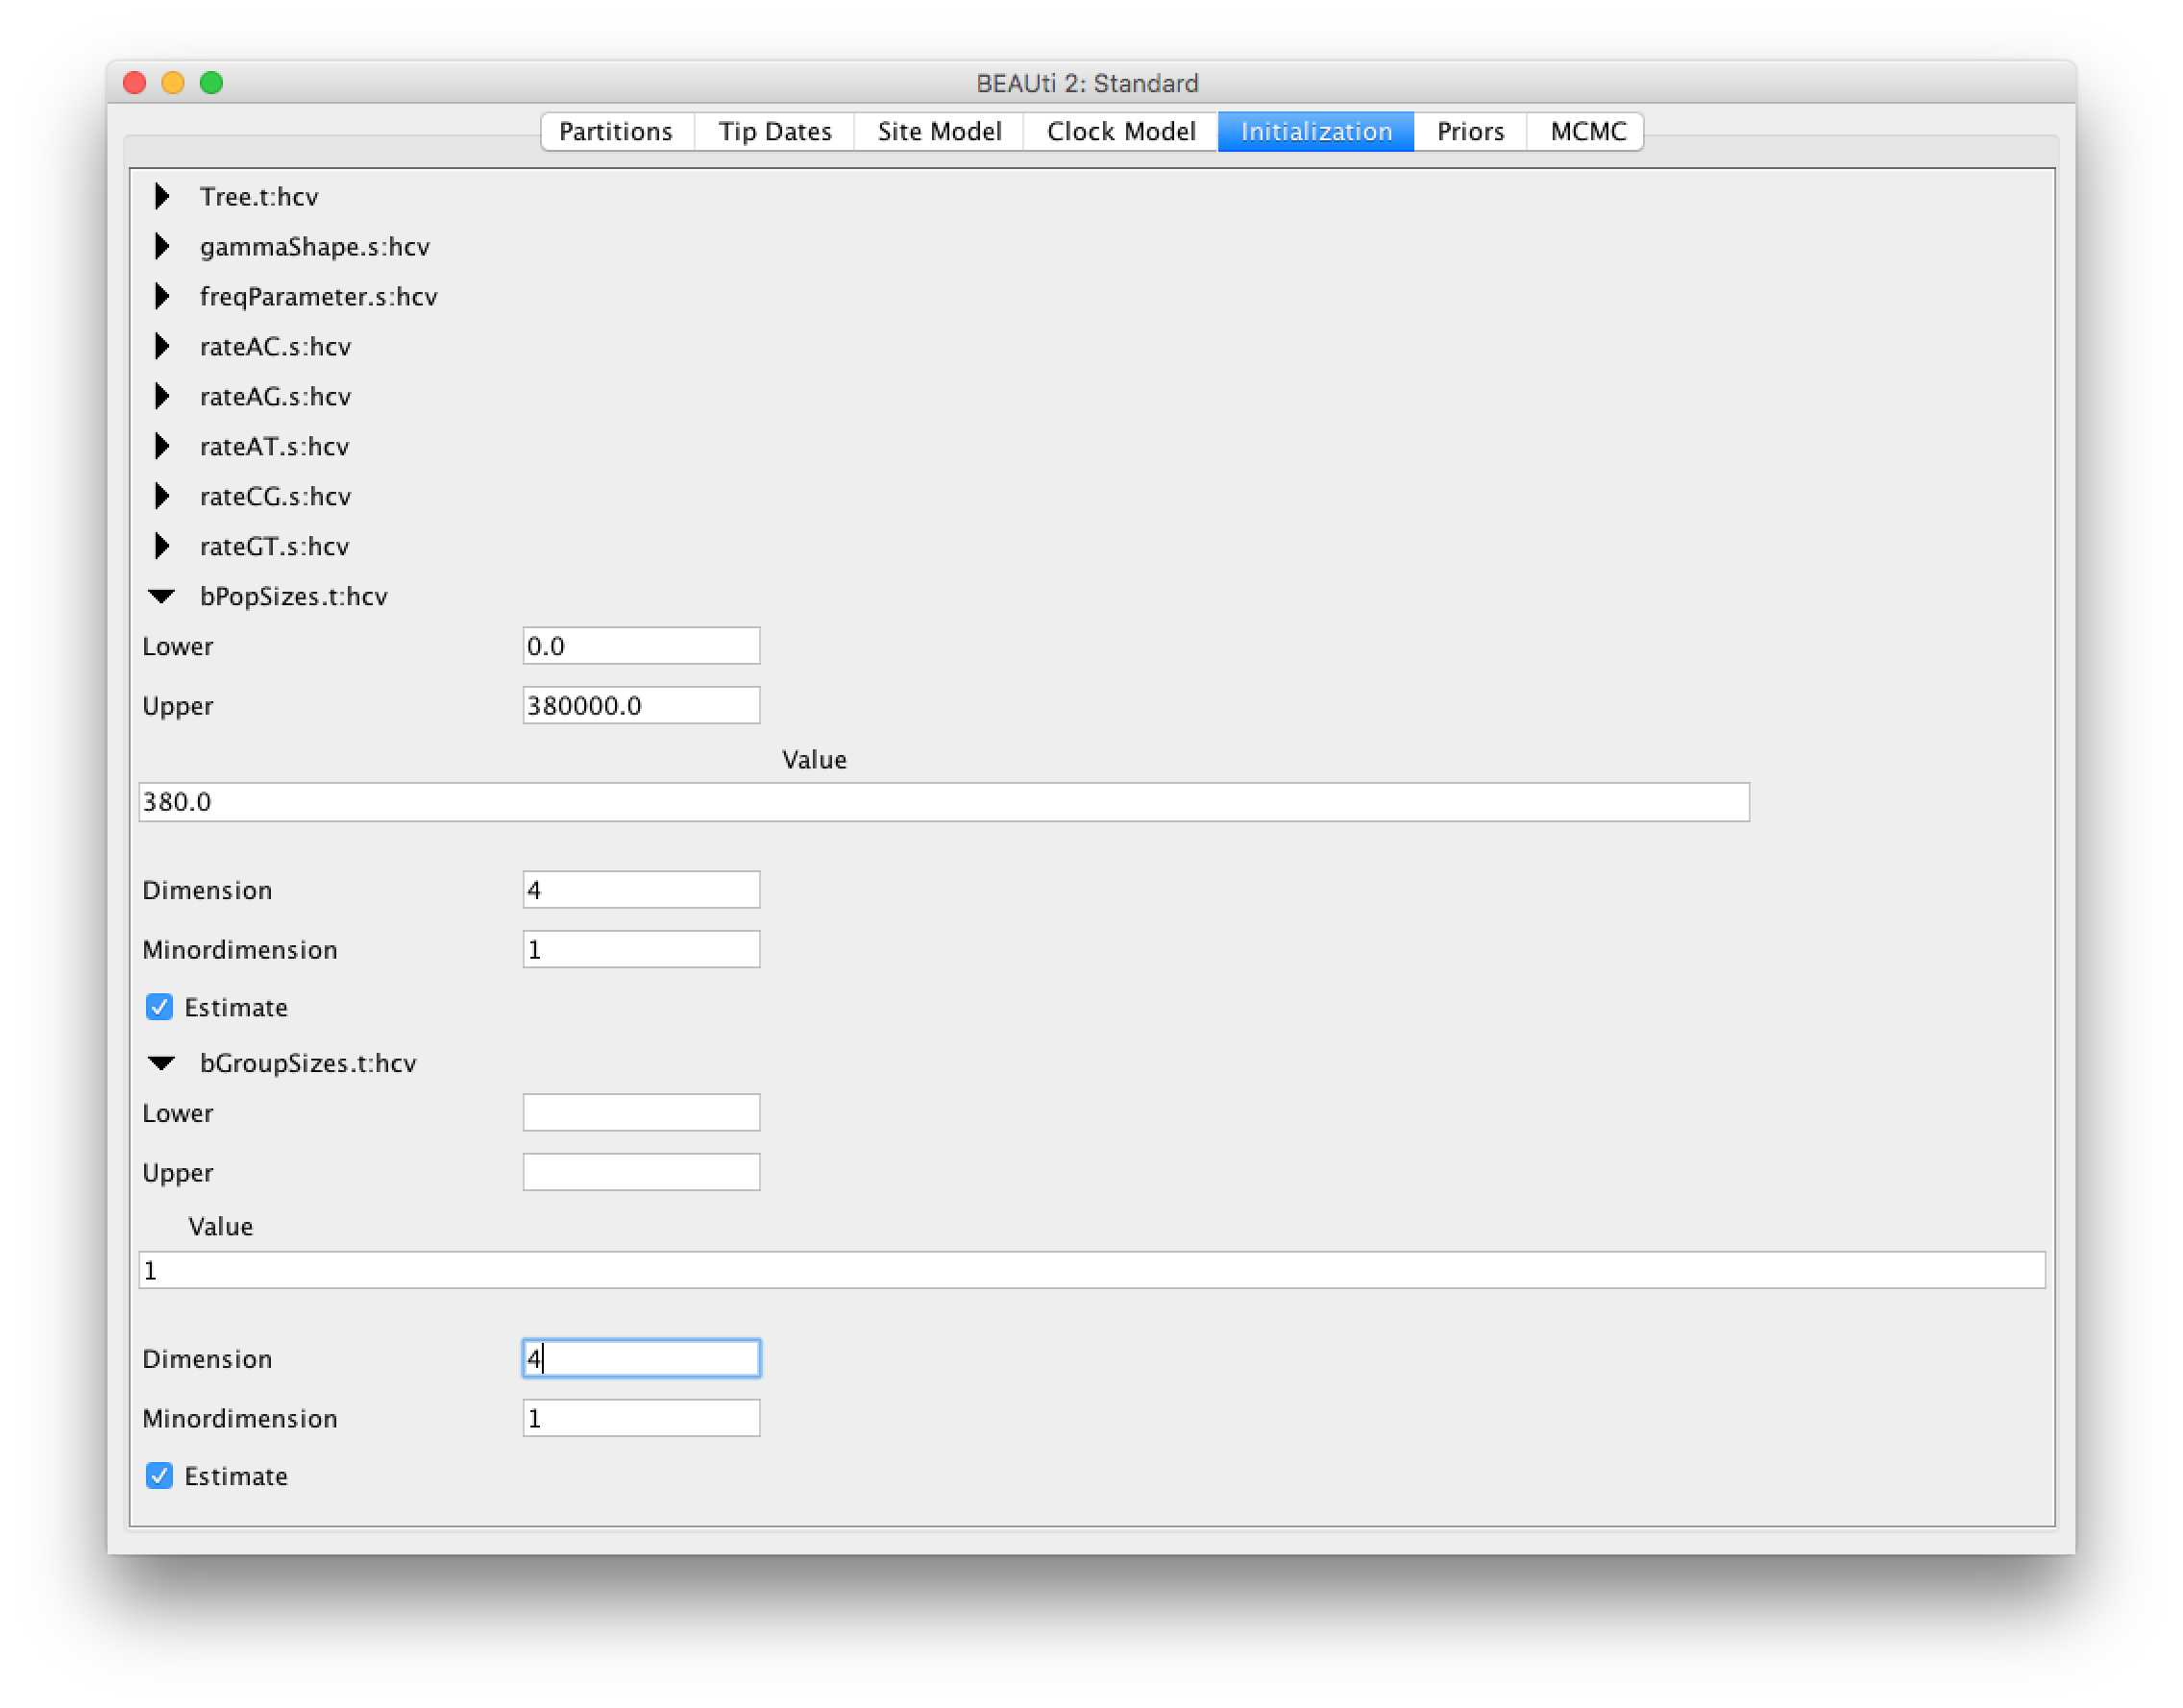
\includegraphics[width=\textwidth]{figures/set_dimension.png}}
\caption{\small Set the dimension of the two parameters, bPopSizes and bGroupSizes, to $4$.}
\label{fig:dimensions}
\end{figure}


Choosing the dimension for the Bayesian Coalescent Skyline can be rather arbitrary. If the dimension is chosen too low, not all population changes are captured, if it is chosen too large, there might be too little information in an interval to support an estimate of a population size. There are implementations in BEAST of the coalescent skyline that either sample dimensions (Extended Bayesian Skyline~\citep{Heled2008}) or do not require dimensions to be specified (Skyride~\citep{Minin2008}).

We can leave the priors as they are and save the settings to *.xml

%The MCMC will now run for a couple of minutes, depending on the speed of the computer. In the meantime, we can open tracer to have a look at the *.log file.

\clearpage

\subsubsection{Effective Population Size}


The effective population size is the inverse of the rate of coalescence $\lambda$. The larger the effective population size N$_{\mathrm{eff}}$ the less likely lineages are to coalesce.

\begin{equation}
\lambda = \frac{1}{\mathrm{N}_{\mathrm{eff}}}
\end{equation} 

For an SIR model (\textbf{S}usceptible, \textbf{I}nfected and \textbf{R}ecovered), it is proportional to the overall population size N and the number of infected I and inverse proportional to the transmission rate $\theta$. 
\begin{equation}
\mathrm{N}_{\mathrm{eff}} = \frac{\mathrm{I}}{\theta} \frac{\mathrm{N}}{\mathrm{S}}
\end{equation} 

Estimates of the effective population size N$_{\mathrm{eff}}$ therefore do not directly tell us something about the number of infected, nor the transmission rate. Changes of e.g. the transmission rate or the number of infected can show in the effective population size (if they do not cancel out).


%A tree can be simplified by only looking at how often coalescent events happen (Figure~\ref{fig:coal_principle}).

\begin{figure}[h!]
\centering
\fbox{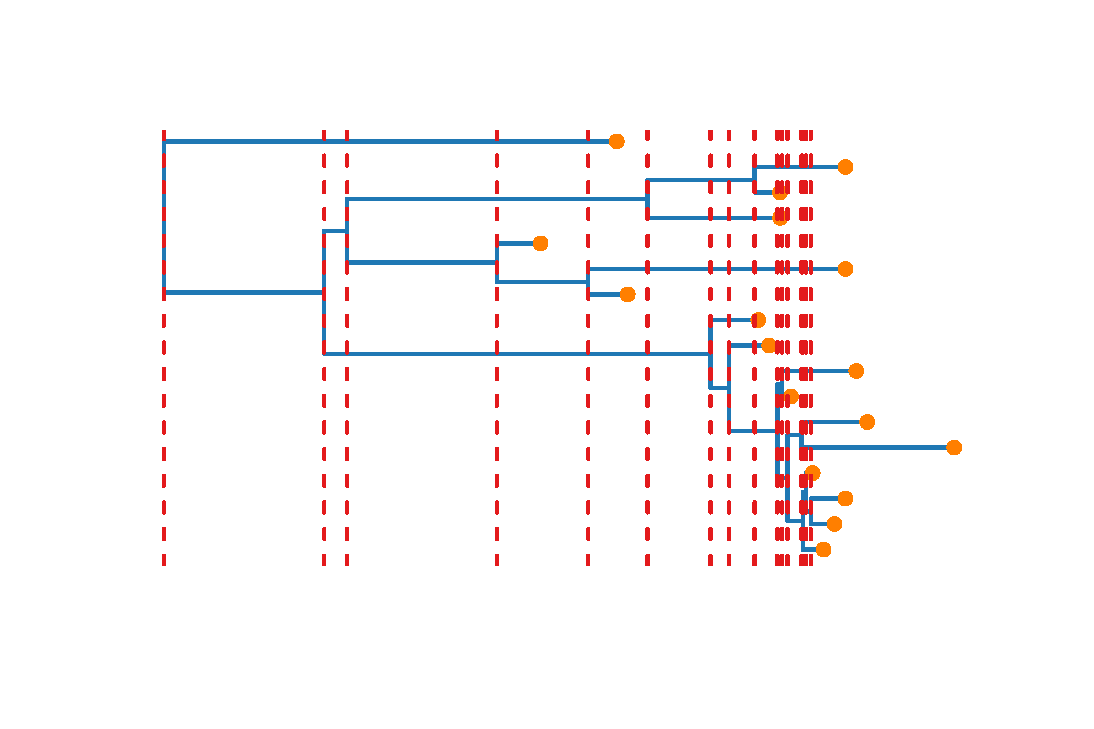
\includegraphics[width=0.6\textwidth]{figures/coalescent_intervals.pdf}}
\caption{\small Example tree where the red dotted lines show the time-points of coalescent events }
\label{fig:coal_principle}
\end{figure}

What the Bayesian Coalescent Skyline is doing is dividing the full tree into dimension $d$ intervals between coalescent events. It then estimates based on what happens in those intervals, what the effective population size is (the actual estimation additionally involves smoothing priors which restrict the difference in effective population sizes between two intervals). The length of an interval is therefore not a fixed value but dependent on where the coalescent events are (Figure~\ref{fig:coal_principle}, compare later to Figure~\ref{fig:bdsky_principle} for the birth-death skyline), as well as the number of events contained within an interval (the GroupSize parameter). Intervals are grouped together, because as Figure~\ref{fig:coal_principle} shows, some of the intervals can be very small, which may lead to erratic estimates. Grouping intervals together leads to smoother estimates.


\subsubsection{Exploring the results of Bayesian Coalescent Skyline analysis}


For the reconstruction of the population dynamics, we need two files: the \texttt{*.log} file and the \texttt{*.trees} file. The log files contain the information about the group size and the population size. The group size specifies how many intervals are combined to have the same effective population size. 

After the runs have finished, load the finished \texttt{*.log} file into Tracer. Alternatively you can use the \texttt{*.log} files and the \texttt{*.trees} files you downloaded with the data. To run the analysis, open the finished \texttt{*.log} file into Tracer, then go to \texttt{Analysis > Bayesian Skyline Reconstruction}. From there open the finished *.trees file. The get the correct years in the analysis we should specify the \texttt{Age of the youngest tip}. In our case it is 1993, the year were all the samples were taken. If the samples were taken through time, the age of the youngest tip is the time when the most recent sample was taken. If you now press the \texttt{Ok} button, the reconstruction of the past population dynamics will be performed (Figure~\ref{fig:trees}).
%\begin{figure}[h!]
%\centering
%\fbox{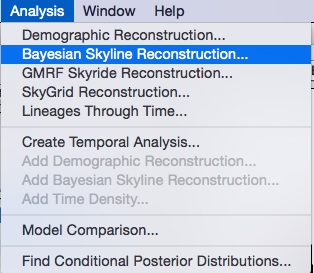
\includegraphics[width=0.3\textwidth]{figures/open_SkylineAnalysis.png}}
%\caption{\small Running Bayesian Skyline reconstruction.}
%\label{fig:recon}
%\end{figure}

\begin{figure}[h!]
\centering
\fbox{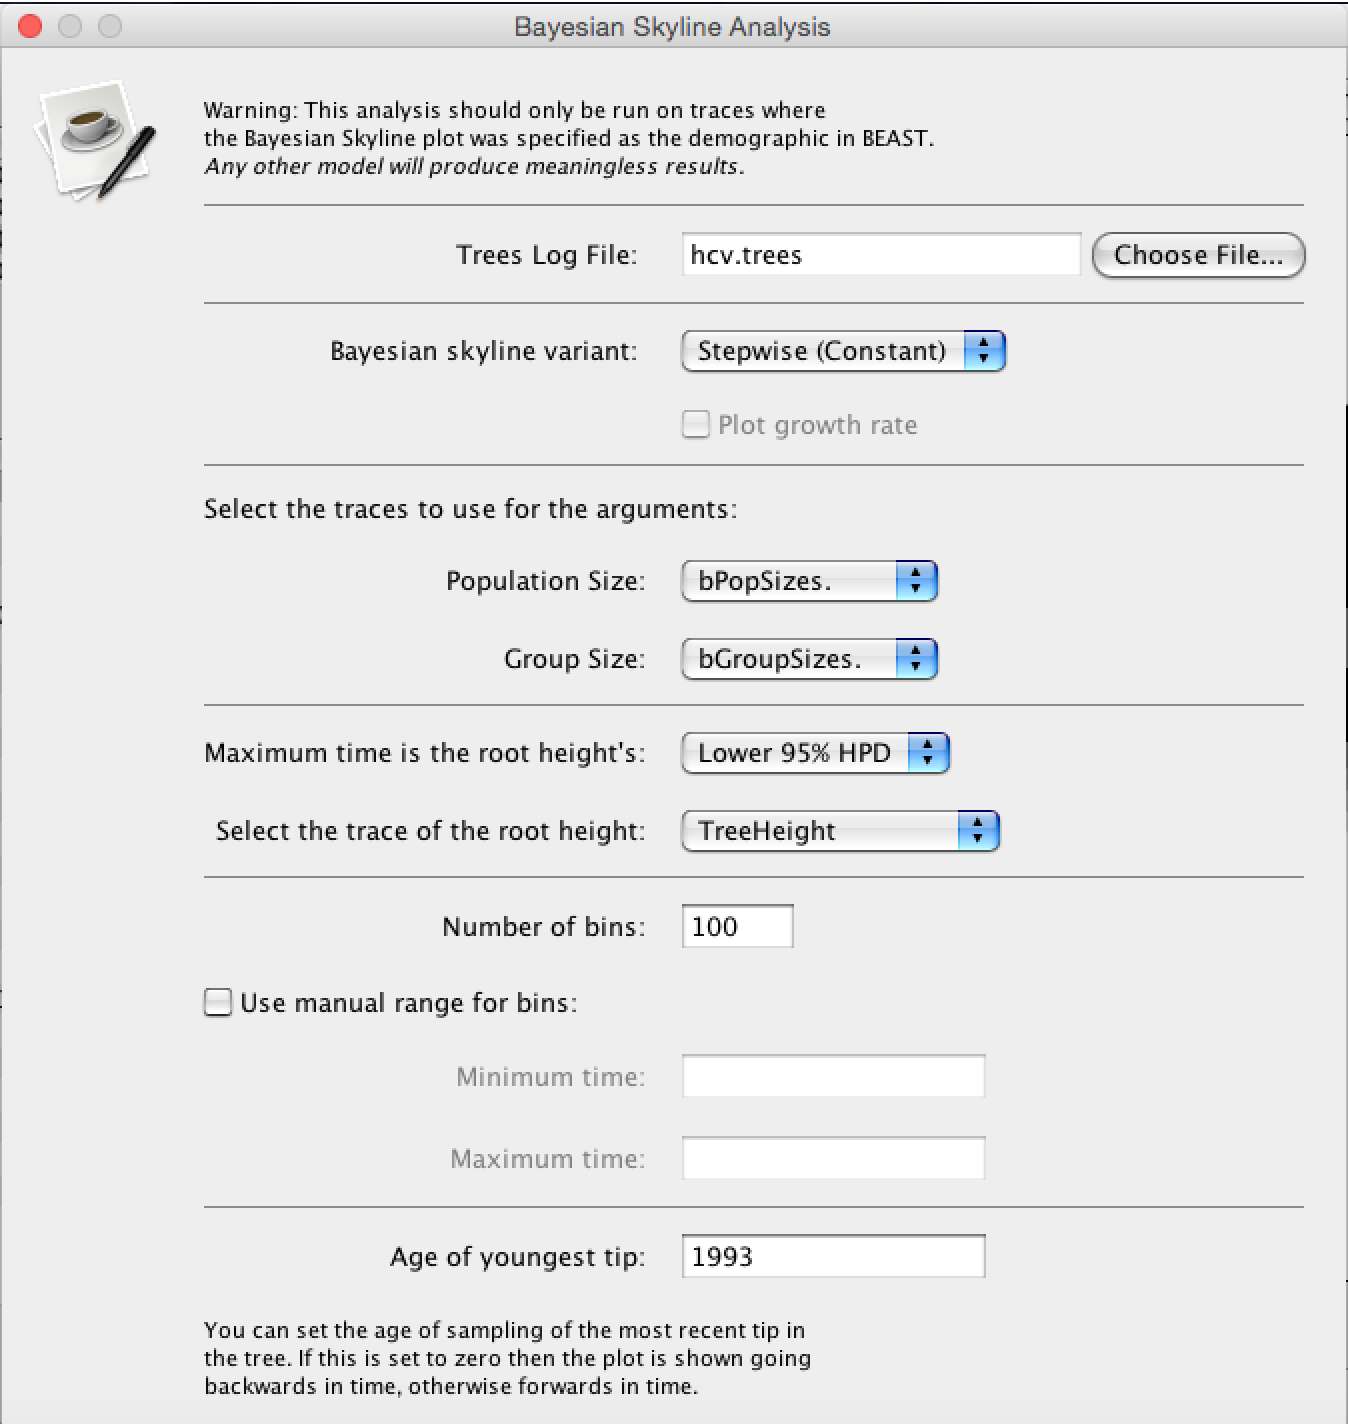
\includegraphics[width=0.6\textwidth]{figures/open_trees.png}}
\caption{\small Reconstructing the Bayesian Skyline plot in Tracer.}
\label{fig:trees}
\end{figure}


%\fixme{it would be better to show the setup in a screenshot rather than %showing how to browse for the tree file again.}
The output will have the years on the $x$-axis and the effective population size on the $y$-axis. By default, the $y$-axis is on a log-scale. If everything worked as it is supposed to work you will see a sharp increase in the effective population size in the mid 20$^{\mathrm{th}}$ century, similar to what is seen on Figure~\ref{fig:skyline}.


\begin{figure}[h!]
\centering
\fbox{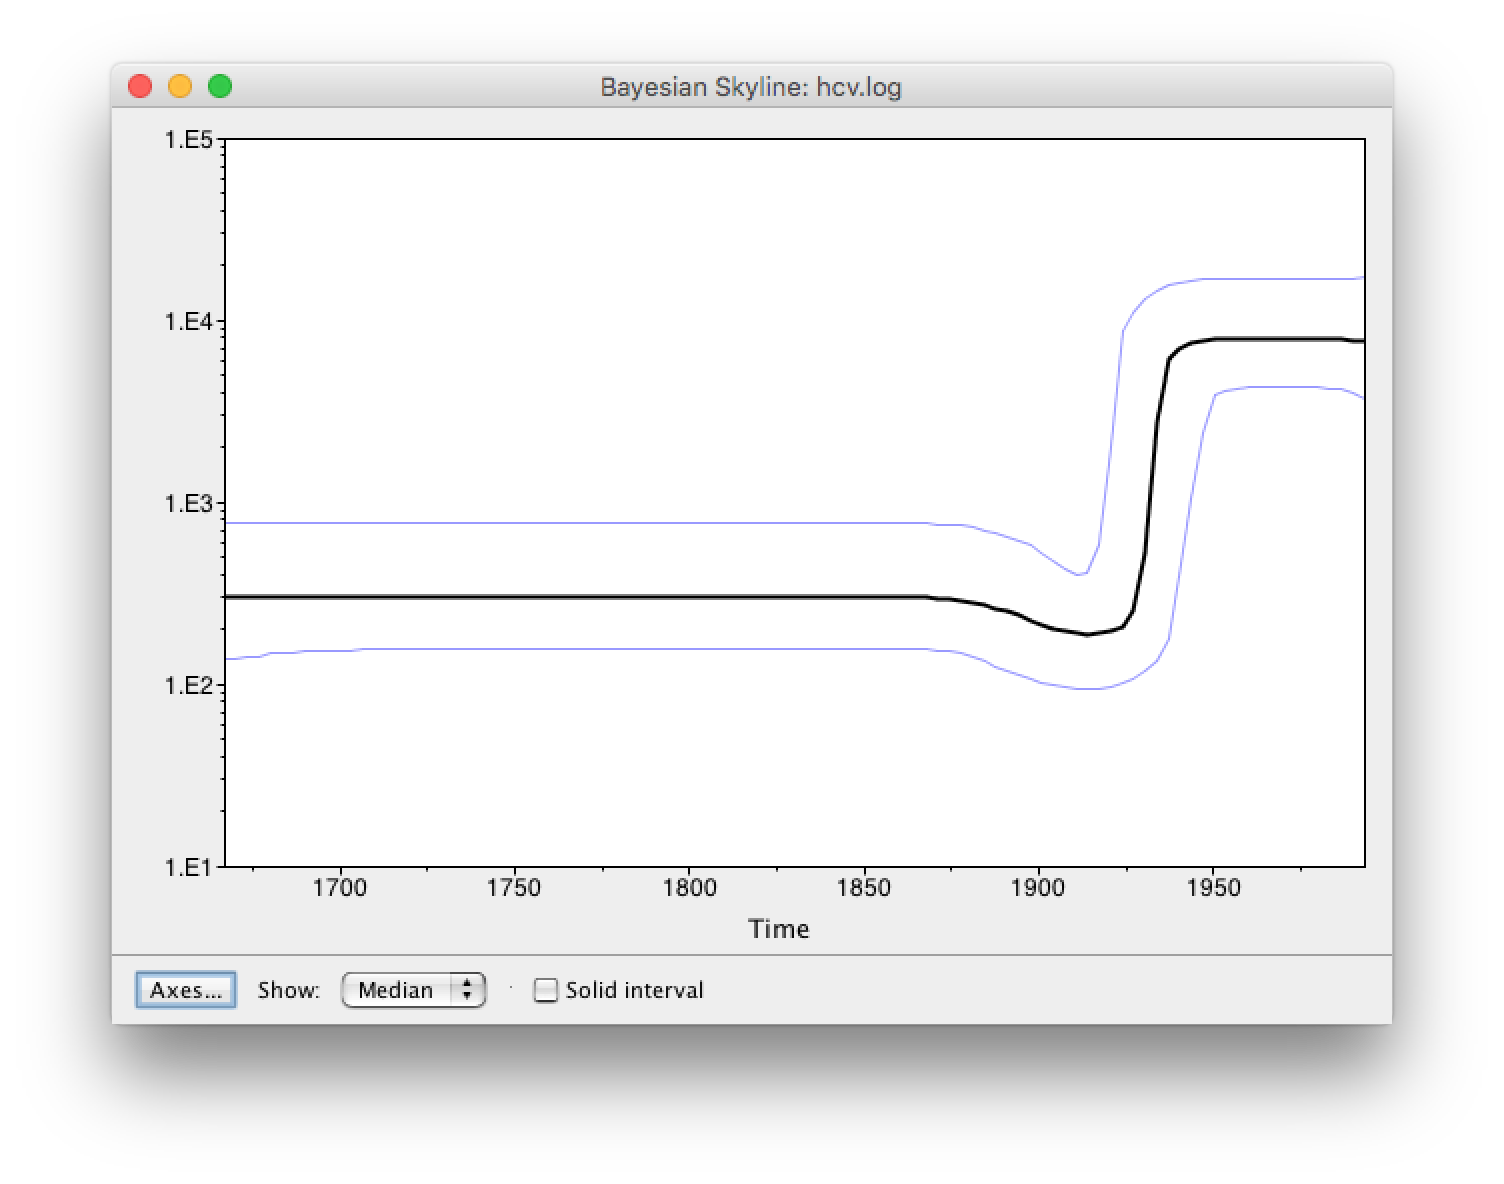
\includegraphics[width=0.6\textwidth]{figures/skyline_analysis.png}}
\caption{\small Bayesian Coalescent Skyline analysis output. The black line is the median estimate of the estimated effective population size (can be changed to the mean estimate). The two blue lines are the upper an the lower estimates of 95$\%$ interval. The x-axis is the time in years}
\label{fig:skyline}
\end{figure}

There are two ways to save the analysis, it can either be saved as a *.pdf or as tab delimited file. To save it as a tab delimited file, you can go to \texttt{File > Export Data}. The exported file will have five rows, the time, the mean, median lower 95$\%$ interval and the upper 95$\%$ interval of the estimates, which you can use to plot the data with other software (R, Matlab, etc).

%\begin{figure}[h!]
%\centering
%\fbox{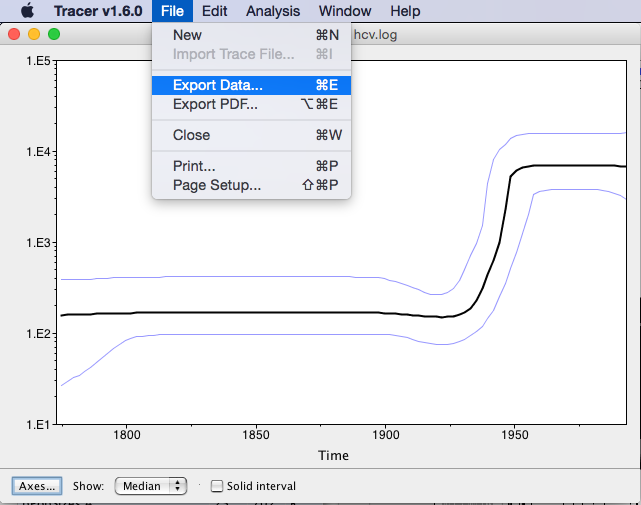
\includegraphics[width=0.6\textwidth]{figures/save_data.png}}
%\caption{\small Saving the result as a tab delimited file.}
%\label{fig:save}
%\end{figure}

\bigskip
\subsubsection{Choosing the Dimension}

%\fixme{Why is this here? Explain it before you run the analysis with 5 dimensions.}
If we compare the estimates of the population dynamics using different dimensions, we see that most of the dynamics are already captured with having only 2 dimensions, as shown in Figure~\ref{fig:comparison}. Adding more dimensions mainly only changes the inferred effective population size before 1900. Note that adding more dimensions adds a slight dip before the increase in the effective population size (around 1900). When comparing to the HPD intervals (Figure~\ref{fig:skyline}) we see that this dip is not significant and may not be indicative of a real decrease in the effective population size before the subsequent increase.

\begin{figure}[h!]
\centering
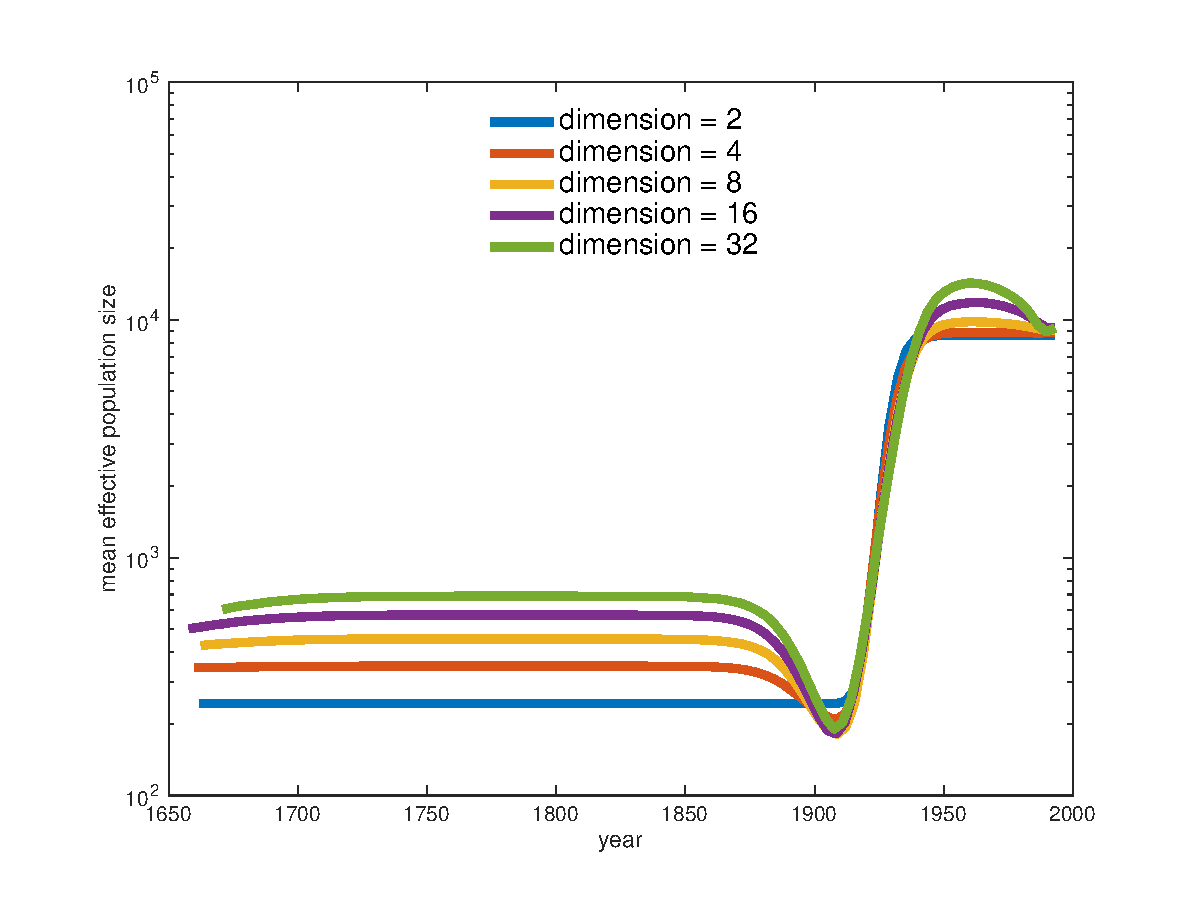
\includegraphics[scale=0.5]{figures/comparison_dimension.eps}
\caption{\small Estimated mean effective population sizes using different dimensions}
\label{fig:comparison}
\end{figure}

The choice of the number of dimensions can also have a direct effect on how fast the MCMC converges (Figure~\ref{fig:ess}). The slower convergence with increasing dimension can be caused by e.g. less information in intervals. To some extent it is simply caused by the need to estimate more parameters though.


\begin{figure}[h!]
\centering
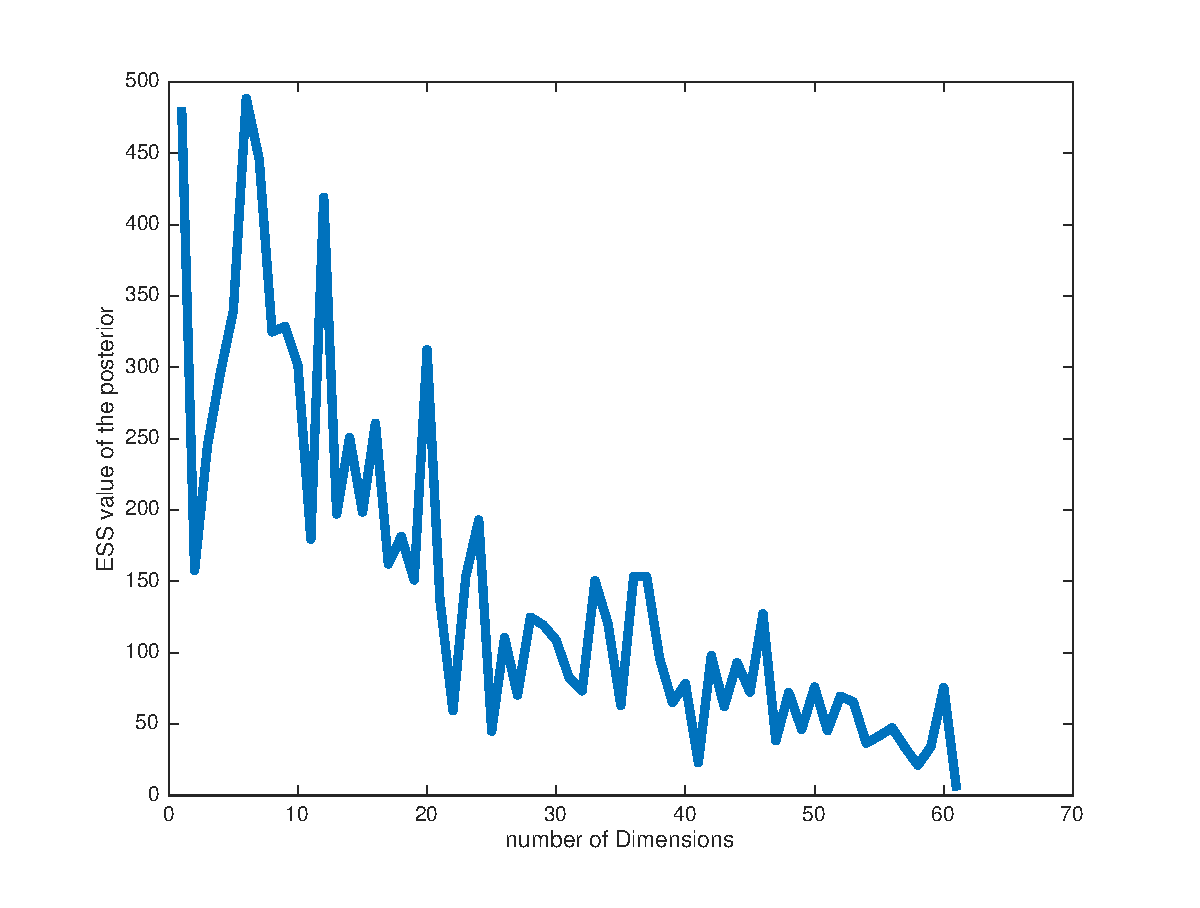
\includegraphics[scale=0.5]{figures/ess_vs_dim_coal.eps}
\caption{\small The ESS value of the posterior after and MCMC with 10$^{7}$ samples, logged every 10$^{3}$ steps and a burnin of 10\% for using different dimensions of the Bayesian Coalescent Skyline}
\label{fig:ess}
\end{figure}

\clearpage
\subsubsection{Birth-Death Skyline}
In the first analysis, we used the coalescent approach to estimate population dynamics, we now want to do the inference using the birth-death skyline model. We will mostly need the same setups as for the previous analysis. In case you closed BEAUti, you can reopen the previously used configuration file in BEAUti (\texttt{File > Load} the *.xml) and modify it to have a birth-death skyline prior on the tree. We will need to set the prior to \texttt{Birth Death Skyline Contemporary}, since the sequences were all sampled at the same point in time (see Figure~\ref{fig:bdsky}). For samples that were taken through time, we would take \texttt{Birth Death Skyline Serial}.

\begin{figure}[h!]
\centering
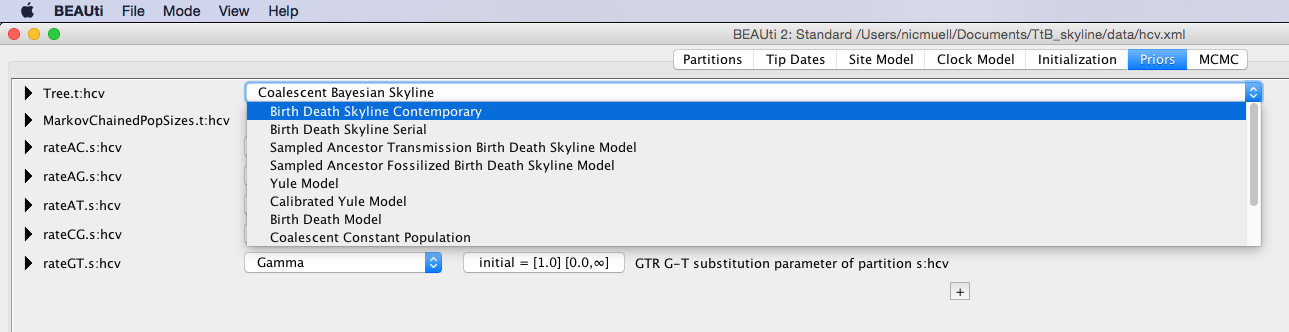
\includegraphics[width=\textwidth]{figures/choose_bdsky.png}
\caption{\small Setting the prior on the tree to the birth-death skyline.}
\label{fig:bdsky}
\end{figure}

As in the Bayesian Coalescent Skyline, we need to choose the number of dimensions. Here we choose the dimensions for the R$_{0}$, the basic reproduction number, which denotes the number of secondary infections caused by a single infected person in a completely susceptible population, i.e. an R$_{0}$ of 2 would mean that every infected person causes two new infections on average. Or in other words, an R$_{0}$ above 1 means that the number of cases are increasing, therefore the disease will cause an epidemic, and an R$_{0}$ below 1 means that the epidemic will die out. (Note that since the birth-death skyline infers changes in R$_0$ over time, it technically infers the effective reproduction number, the average number of new infections caused by an infected person at a certain time during the outbreak).

The dimension of the R$_{0}$ has to be chosen in the initialization panel. Choosing this dimension can again be arbitrary and may require the testing of a few different values. Too few intervals and not all rate shifts are captured. Too many intervals and the intervals may not contain enough information to infer parameters.

%\fixme{why these dimensions? Explain how to set these and where.}
In this case we will keep the default value of 10 dimensions (Figure~\ref{fig:dimensions_bdsky})

\begin{figure}[h!]
\centering
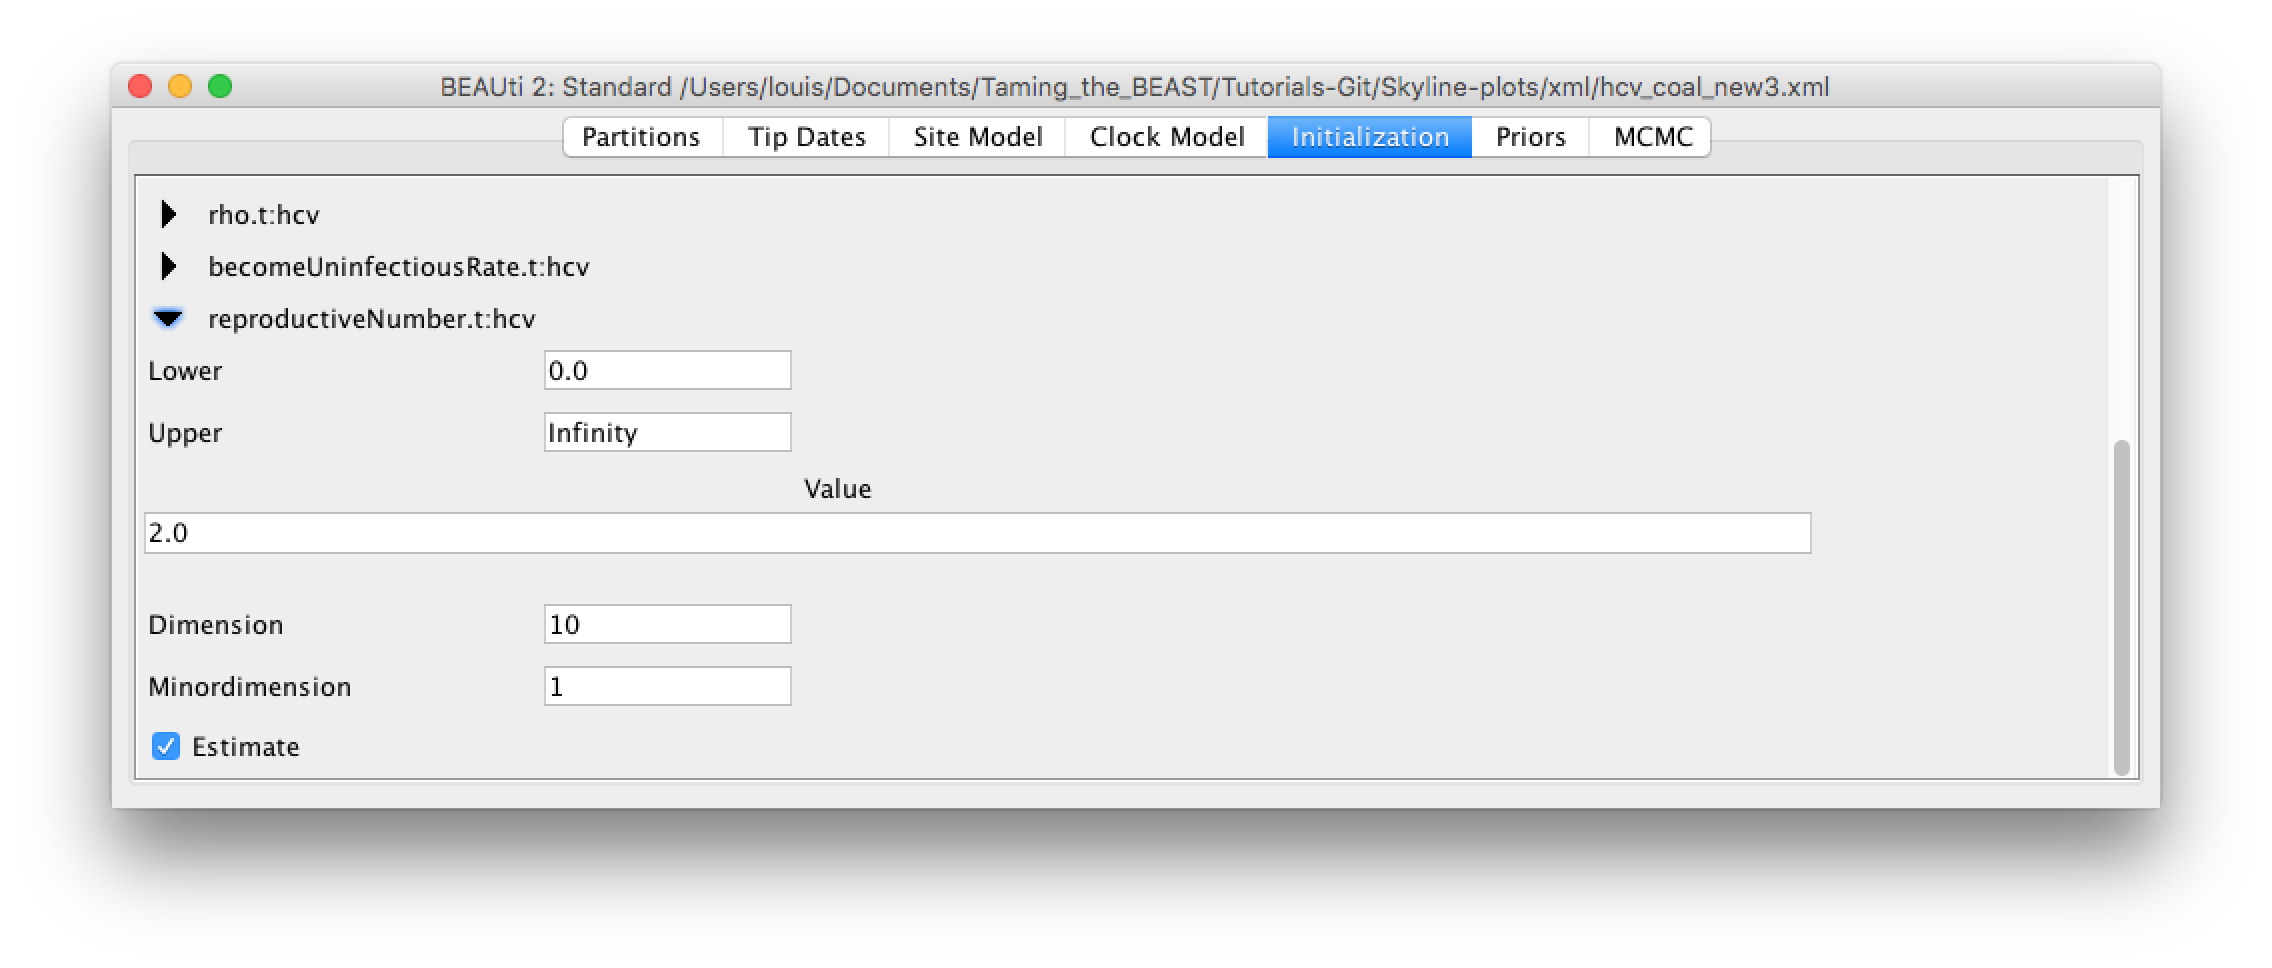
\includegraphics[width=\textwidth]{figures/choose_dimension_bdsky.png}
\caption{\small Setting the dimensions for R$_0$ estimates.}
\label{fig:dimensions_bdsky}
\end{figure}


%\fixme{What does model-based mean? Parametric?}

%\fixme{What is rho?}

%\fixme{Explain all the priors! Where did they come from, why do you set them like this, etc.}


\begin{figure}[h!]
\centering
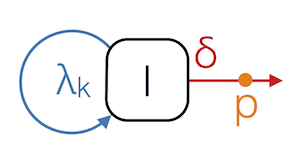
\includegraphics[width=0.25\textwidth]{figures/bdsky_model.png}
\caption{\small A schematic of the BDSky model}
\label{fig:bdsky_model}
\end{figure}

BDSKY infers 3 parameters (Figure~\ref{fig:bdsky_model}), the transmission rate $\lambda$, the becoming noninfectious rate $\delta$ and the sampling proportion, $\rho$ (when the samples were taken at the same time) or the sampling proportion, $p$ (when the samples were taken through time). The R$_{0}$ is then a function of those values (more about that later).
The rates we estimate using the birth-death model are per lineage rates. Some of these rates we know or we can estimate them from other data. The becoming noninfectious rate for example, we can get from the average time a patient can transmit a disease. This prior knowledge we can incorporate in the MCMC.
This we can do in the \texttt{Priors} panel. We can use prior information about the R$_{0}$, the becoming noninfectious rate, the origin and rho (Figures~\ref{fig:r0prior},~\ref{fig:bURprior},~\ref{fig:oriprior},~\ref{fig:rhoprior}). Note that the origin inferred by the birth-death skyline is not the time of the most recent common ancestor of the tree (MRCA), but is earlier and denotes the start of the outbreak, i.e. when there was only one infected person. 


%\fixme{justify priors}

We use a lognormal prior for $R_0$. This is a good prior distribution to use for rates since it is always positive (a rate cannot be negative) and has a long tail defined over all positive numbers. The long tail allows arbitrarily high estimates of $R_0$, but does not place much weight on very high rates. This agrees with our prior knowledge about the $R_0$ of other diseases (most diseases have an $R_0$ between 1.2 and 5. Measles is one of the most infectious diseases we know about and has an $R_0$ of around 18). 

If an epidemic is neither growing nor declining, it has an R$_{0}$ of 1, which we will use as a null hypothesis (we assume that as long as there is no strong signal in an interval for an epidemic to grow or decline that the R$_{0}$ is 1, i.e. the epidemic stays constant). Thus, we set the mean of the lognormal distribution to 0, which results in a median of 1. We set the variance to 1.25, which places most weight below 7.82 (95\% quantile). (Figure~\ref{fig:r0prior}).

\begin{figure}[h!]
\centering
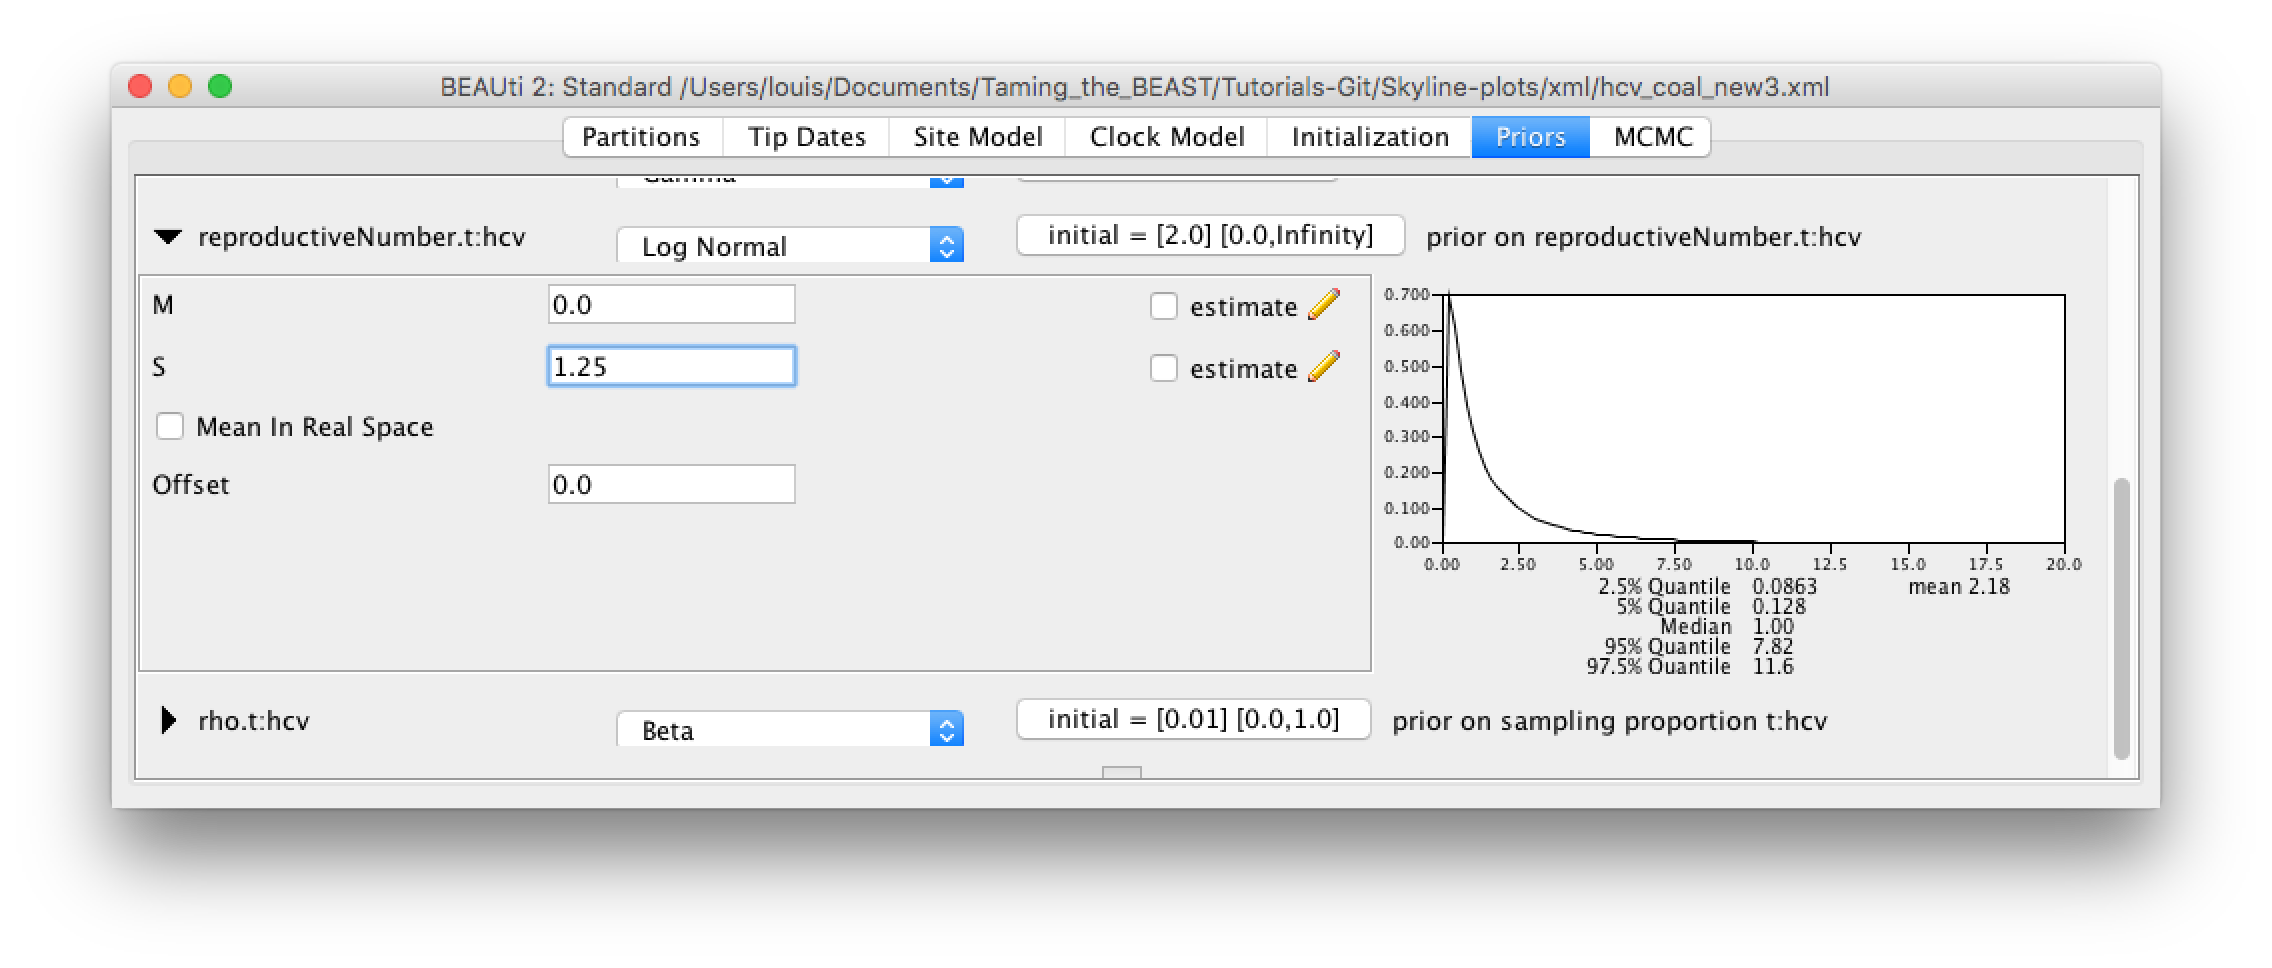
\includegraphics[width=\textwidth]{figures/bdsky_prior_r0.png}
\caption{\small Setting the R$_{0}$ prior.}
\label{fig:r0prior}
\end{figure}

For the becoming noninfectious rate we again use a lognormal prior. The inverse of the becoming noninfectious rate is the average infectious period. In some patients an HCV infection only lasts a few weeks, while in others it is a chronic infection lasting for many years. Setting $M=0$ and $S=1.25$ results in the same prior we used for the $R_0$ (Figure~\ref{fig:bURprior}).  In terms of the becoming noninfectious rate, this translates to the 95\% quantiles for the infectious period falling between 0.128 years (46.67 days) and 11.59 years, with a median of 1 year. We will see later that there is a strong signal in the data for a longer becoming noninfectious period. 

\begin{figure}[h!]
\centering
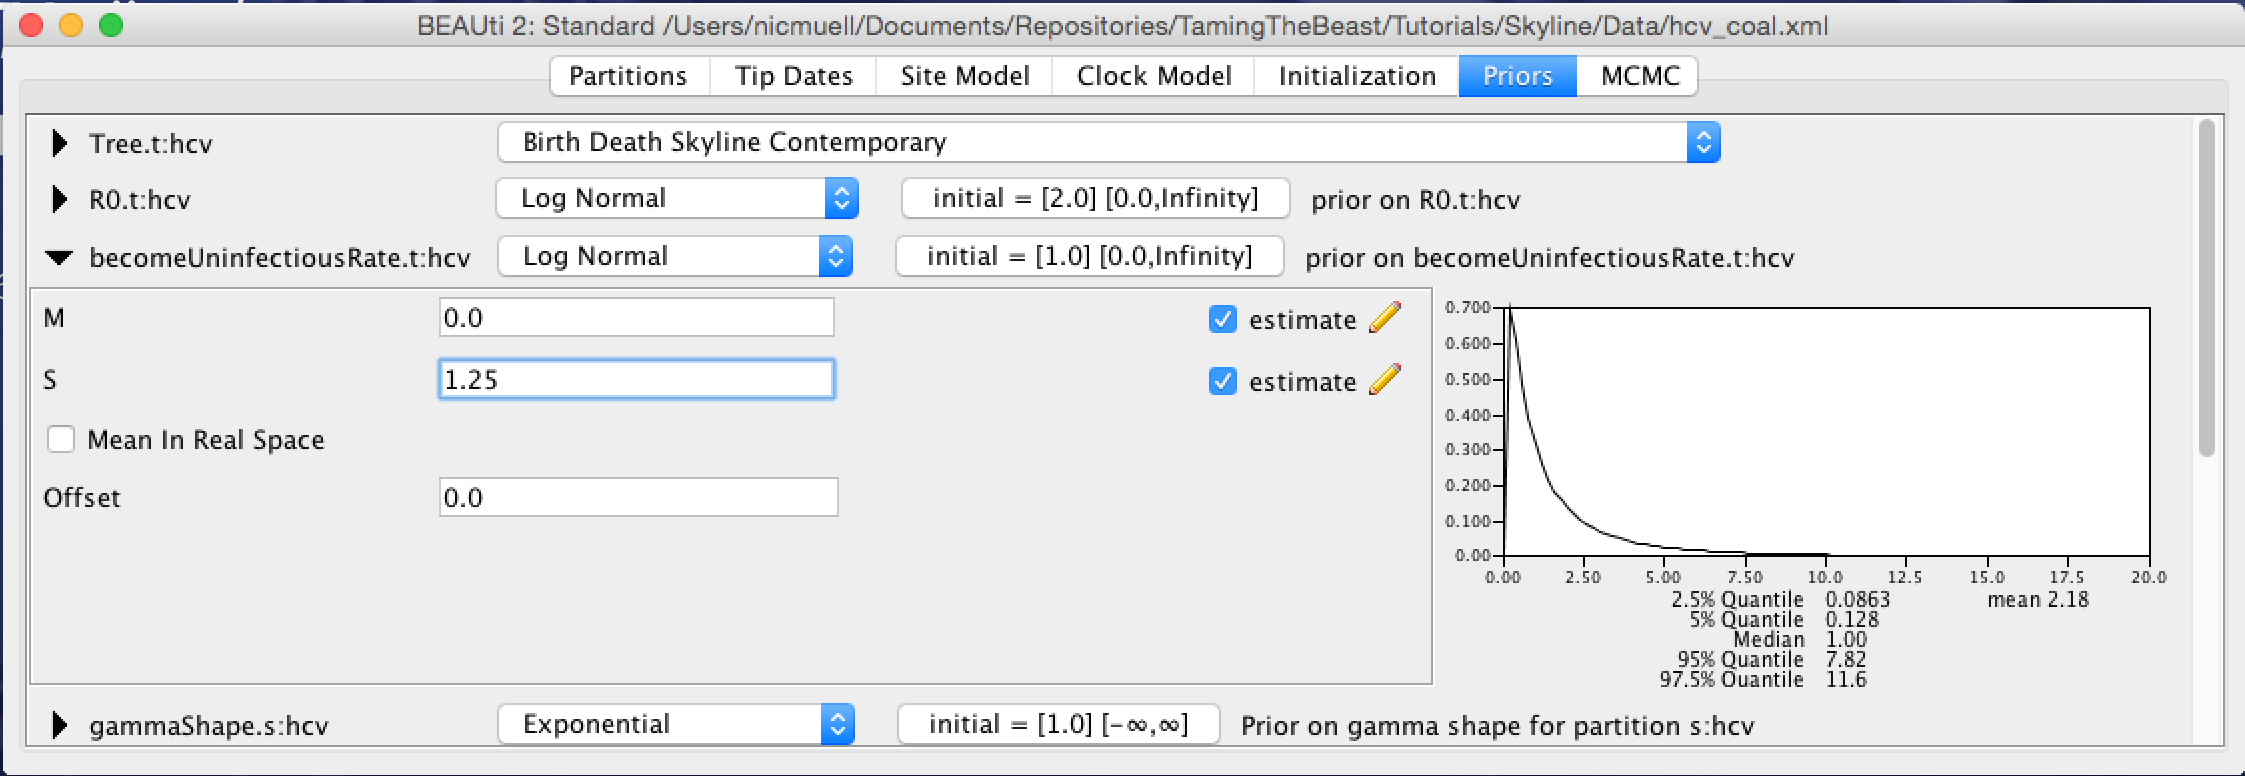
\includegraphics[width=\textwidth]{figures/bdsky_prior_uninf.png}
\caption{\small Setting the becoming noninfectious prior.}
\label{fig:bURprior}
\end{figure}

For the origin of the epidemic we once again use a lognormal prior. Note that the origin also has to be positive and needs to be bigger than the MRCA of the tree. We know that HCV has been circulating in Egypt for at least a hundred years, so we set $M=5$ and $S=0.5$ (Figure~\ref{fig:oriprior}), resulting in a median prior estimate for the origin of 148 years.


\begin{figure}[h!]
\centering
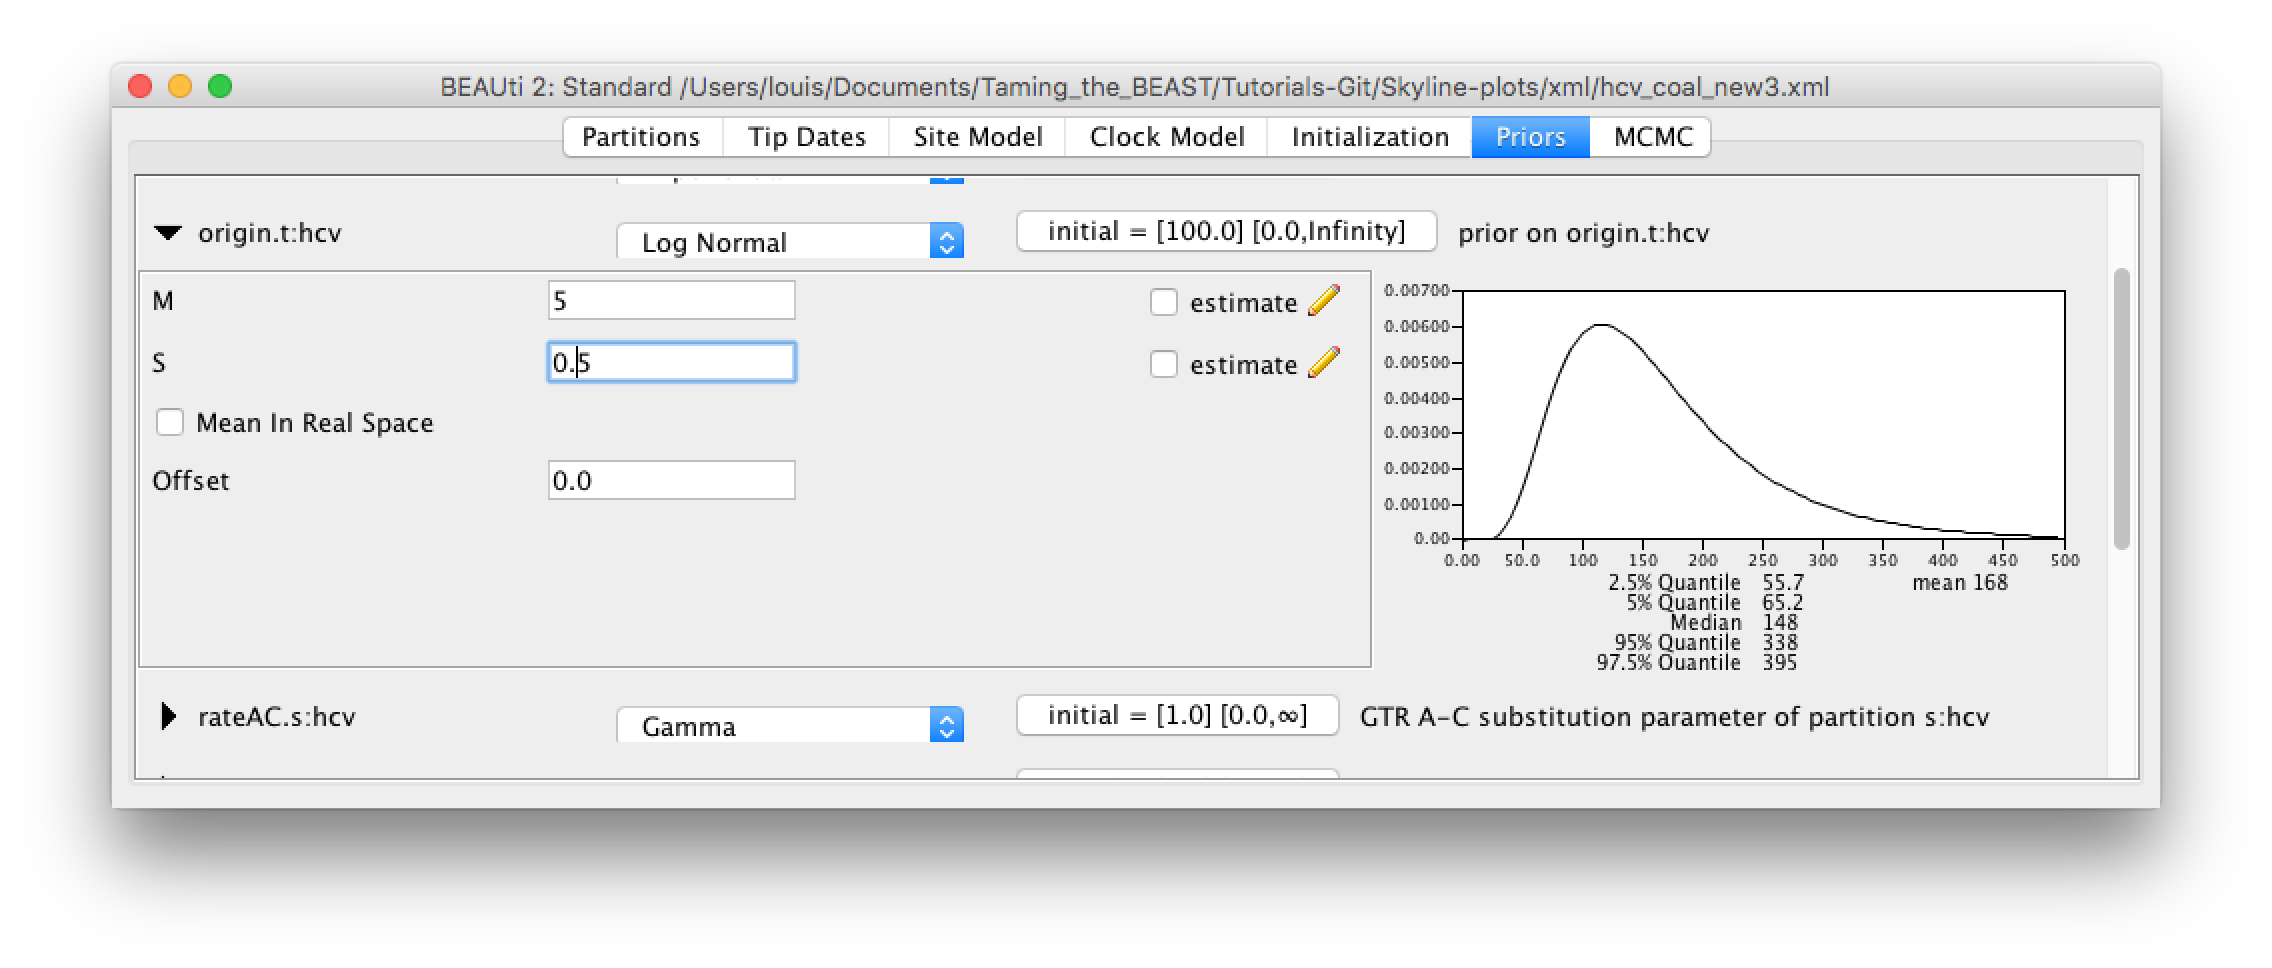
\includegraphics[width=\textwidth]{figures/bdsky_prior_ori.png}
\caption{\small Setting the prior on the origin of the epidemic.}
\label{fig:oriprior}
\end{figure}

Finally, we need a prior for the sampling probability, $\rho$, which represents the proportion of HCV cases in Egypt in 1993, included in the analysis. Egypt had a population of roughly 60 million in 1993, and with a prevalence of at least 15\% this translates into millions of cases, whereas we have only 63 sequences. 

We use a beta distribution for the prior on $\rho$. Beta distributions are a very flexible class of distributions that are only defined between 0 and 1, making them ideal to use for proportions. We set Alpha to 1 and Beta to 9999, reflecting our prior knowledge that we have only a minuscule fraction of all cases in our dataset (Figure~\ref{fig:rhoprior}).

\begin{figure}[h!]
\centering
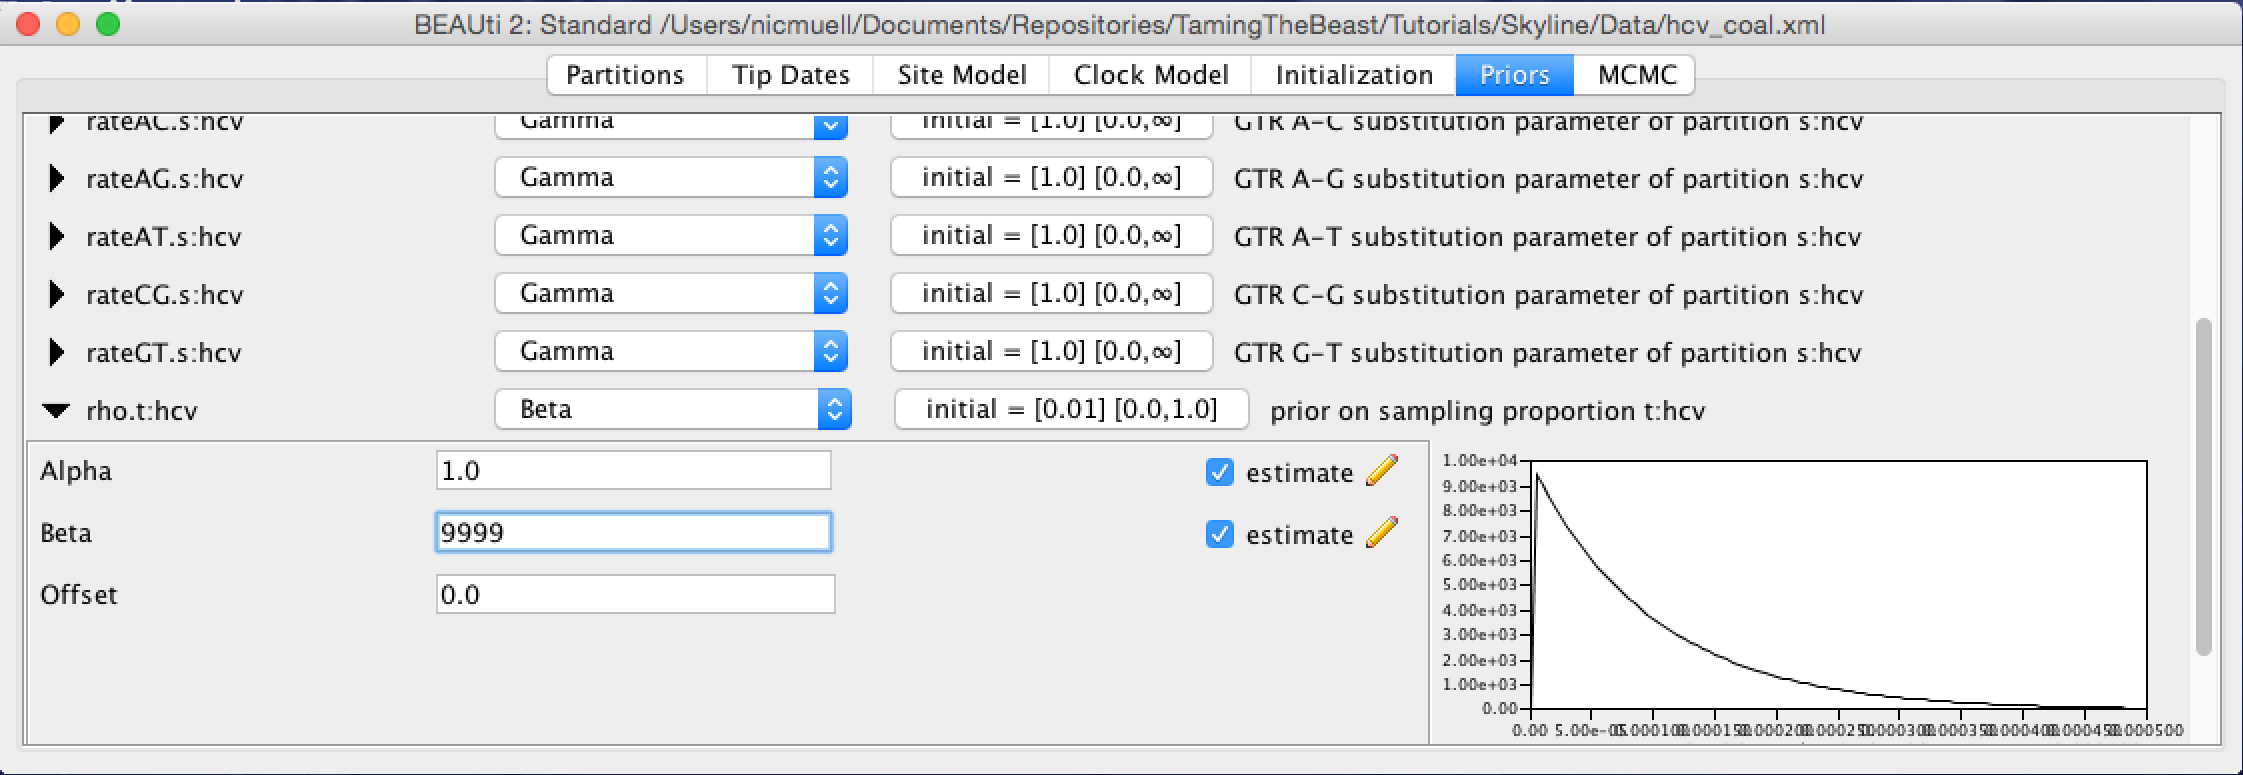
\includegraphics[width=\textwidth]{figures/bdsky_prior_rho.png}
\caption{\small Setting the prior on rho.}
\label{fig:rhoprior}
\end{figure}

We can leave the rest of the priors as they are. First, we should increase the chain length (at least double it). To not get too large log files, we can increase the \texttt{sampling every} to 2000 (reducing the sampling frequency). Now we can change the names of the output files. If we want to run the analysis in the same directory as the coalescent analyses, the output files and the \texttt{*.xml} name need to be different.

\clearpage

%\fixme{What do you mean by the first sentence in this paragraph?}

%\fixme{You just set two different priors for rho and become uninfectious rate and now you're saying it is the same thing. Also there's no rho on the model figure at all, there's a delta which denotes bUR. Re-read and explain this properly!}

%In the meantime, we can have a look at what the birth-death-skyline plot is doing. BDSKY has 3 main parameters: the transmission rate $\lambda$, the sampling rate p and the becoming un-infectious rate $\delta$ (see Figure~\ref{fig:bdsky_model} for a schematic view of the model).



%\fixme{Did you set the bUR dimension to 1? Is it done by default? Explain!}

%\fixme{Explain last sentence. Why don't we need to estimate the sampling probability if there's no sampling through time?}



\subsubsection{The parameterization of the Birth-Death Model}

The Birth-Death model is parameterized very differently from the coalescent model. While the coalescent uses the effective population size, which as the name already tells us is defined on a population level, the birth-death model uses per lineage rates. The transmission rate $\lambda$ tells us at which rate infected individuals infect susceptibles. This rate is also referred to as the birth rate. The sampling rate $\psi$ and the sampling probability $\rho$ describe how likely it is for an infected individual to be sampled and therefore how likely they are to appear in the tree as tips. The becoming noninfectious rate $\delta$ is the sum of the death rate $\mu$ and the sampling rate $\psi$.
\begin{equation}
\delta = \psi + \mu
\end{equation}
The death rate $\mu$ is the rate at which lineages disappear (go extinct) from a population without being sampled. You can also see from the above equation that we assume that a sampled lineage cannot transmit anymore. The consequence for the phylogeny is that a sampled lineage can not be an ancestor of any lineage. This assumption can be relaxed, but we will not do so during this tutorial.
%There are methods that do not make this assumption and allow for sampled ancestors~\citet{Gavruskina}\fixme{citation} 

The R$_{0}$ we estimate is then defined as follows:
\begin{equation}
R_{0} = \frac{\lambda}{\psi + \mu} = \frac{\lambda}{\delta}
\end{equation}
\begin{eqnarray*}
& \text{if} \ \lambda > \delta \ \text{then} \ R_{0} > 1 & \text{epidemic grows}\\
& \text{if} \ \lambda = \delta \ \text{then} \ R_{0} = 1 & \text{epidemic stays constant}\\
& \text{if} \ \lambda < \delta \ \text{then} \ R_{0} < 1 & \text{epidemic declines}
\end{eqnarray*}

The birth-death skyline allows these rates to change over time. This is done by dividing the time from the origin (of the epidemic, which is not necessary the same as the root of the tree) to the most recent sample into dimension $d$ equally spaced intervals (see Figure~\ref{fig:coal_principle}). The rates are then allowed to change between two intervals. Within an interval rates are constant. In principle, all rates in all intervals could be different. Since the transmission rate and the becoming noninfectious rate are highly correlated, this is not always practical. Often we assume the becoming noninfectious rate to be the same in all intervals while changing the transmission rate $\lambda$. 

\begin{figure}[h!]
\centering
\fbox{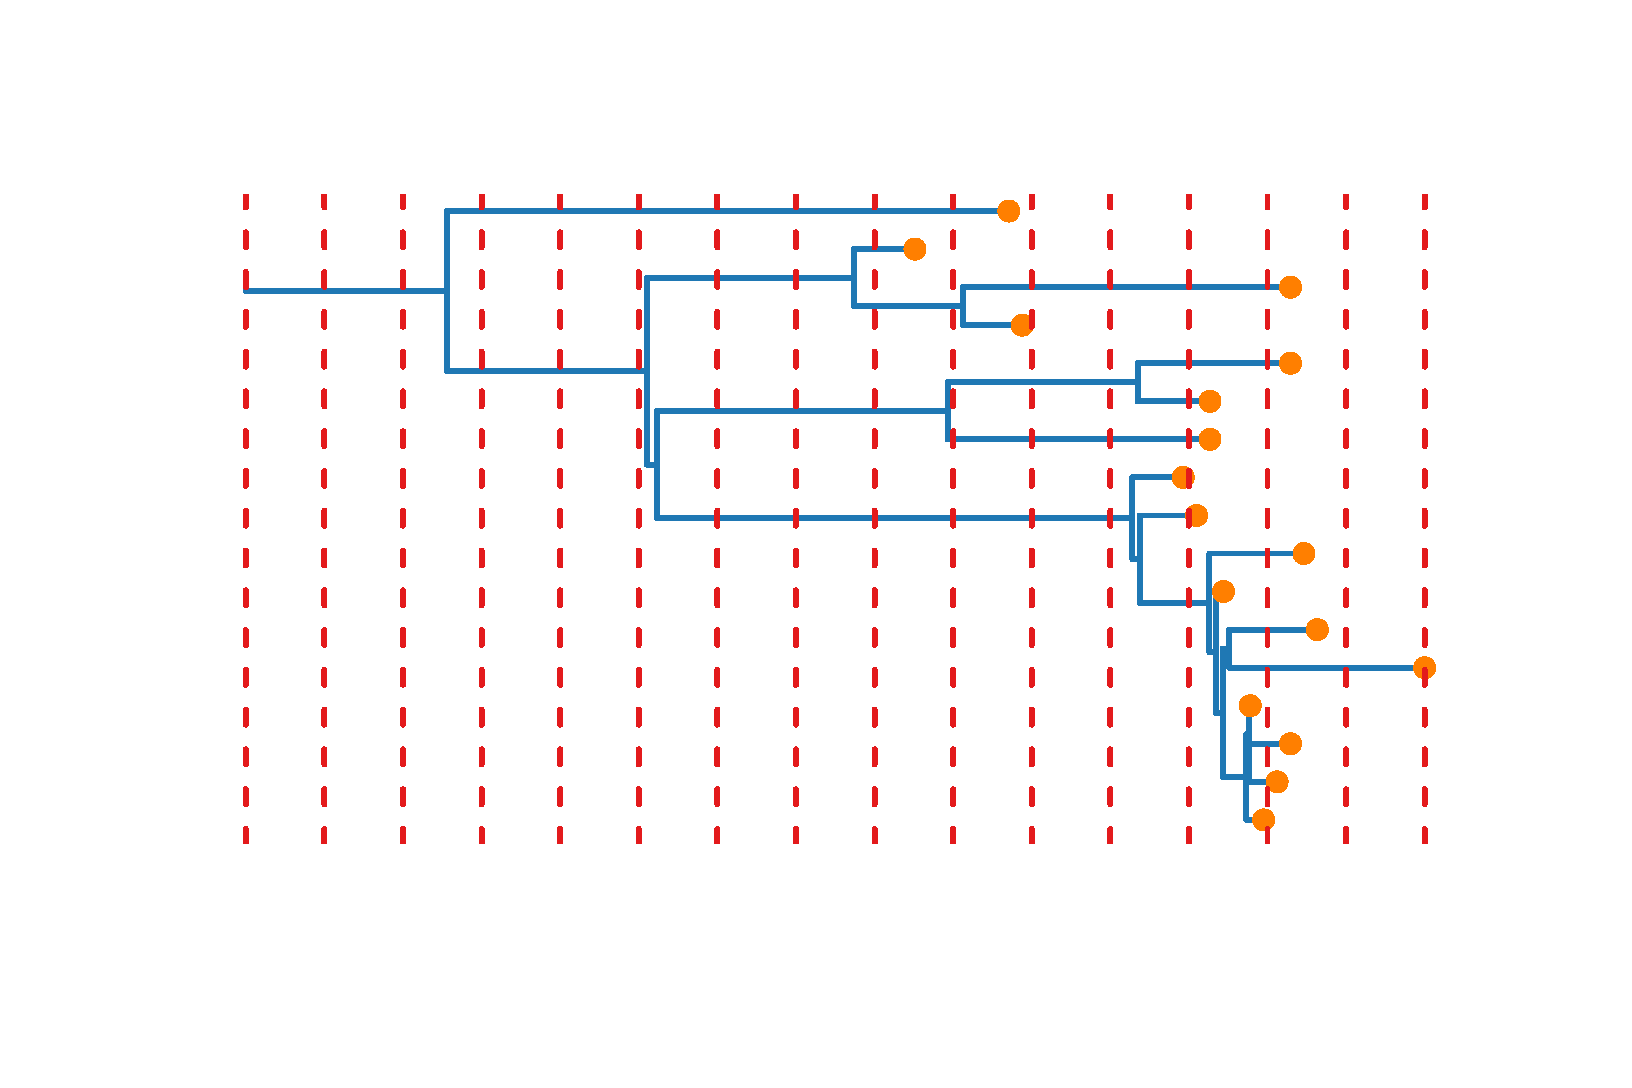
\includegraphics[width=0.6\textwidth]{figures/bdsky_intervals.pdf}}
\caption{\small Example tree where the red dotted lines are an example of where rates could be allowed to change on the tree. The branch at the root (compare Figure~\ref{fig:coal_principle}) is indicating the origin of the epidemic, which is also estimated in the BDSKY.}
\label{fig:bdsky_principle}
\end{figure}

There are some clear differences between the birth-death and the coalescent skyline. First, the way intervals are defined. In the coalescent skyline, intervals are always between coalescent events, while this restriction does not exist for the birth-death skyline. Second, the birth-death skyline does not infer changes in population sizes.
% Not sure what this is
%\begin{equation}
%R_{0} = \frac{\delta I}{\delta t}
%\end{equation}
The coalescent on the other hand does infer the effective population size, which is a parameter proportional to absolute sizes. The third difference is the inference of the origin of an epidemic by the birth death model, which is not done by the coalescent.


\subsubsection{Visualize the Birth-Death Skyline Output}

There is no equivalent visualization of the \texttt{*.log} file of a BDSKY analysis in tracer as there is for the Bayesian Coalescent Skyline. But because BDSKY separates the full tree into equally spaced intervals, we can already get an idea of the inference just by looking at the inferred $R_{0}$ values (see Figure~\ref{fig:bdsky_dynamics}). This gives us a good idea of the trend, but it is not completely accurate. Since every posterior sample has a different origin, the time spanned by each interval is slightly different in each posterior sample. Thus, the different intervals overlap slightly. The advantage to this is that we get a smooth estimate through time. The disadvantage is that we need to do some extra post-processing to plot the skyline.

\begin{figure}[h!]
\centering
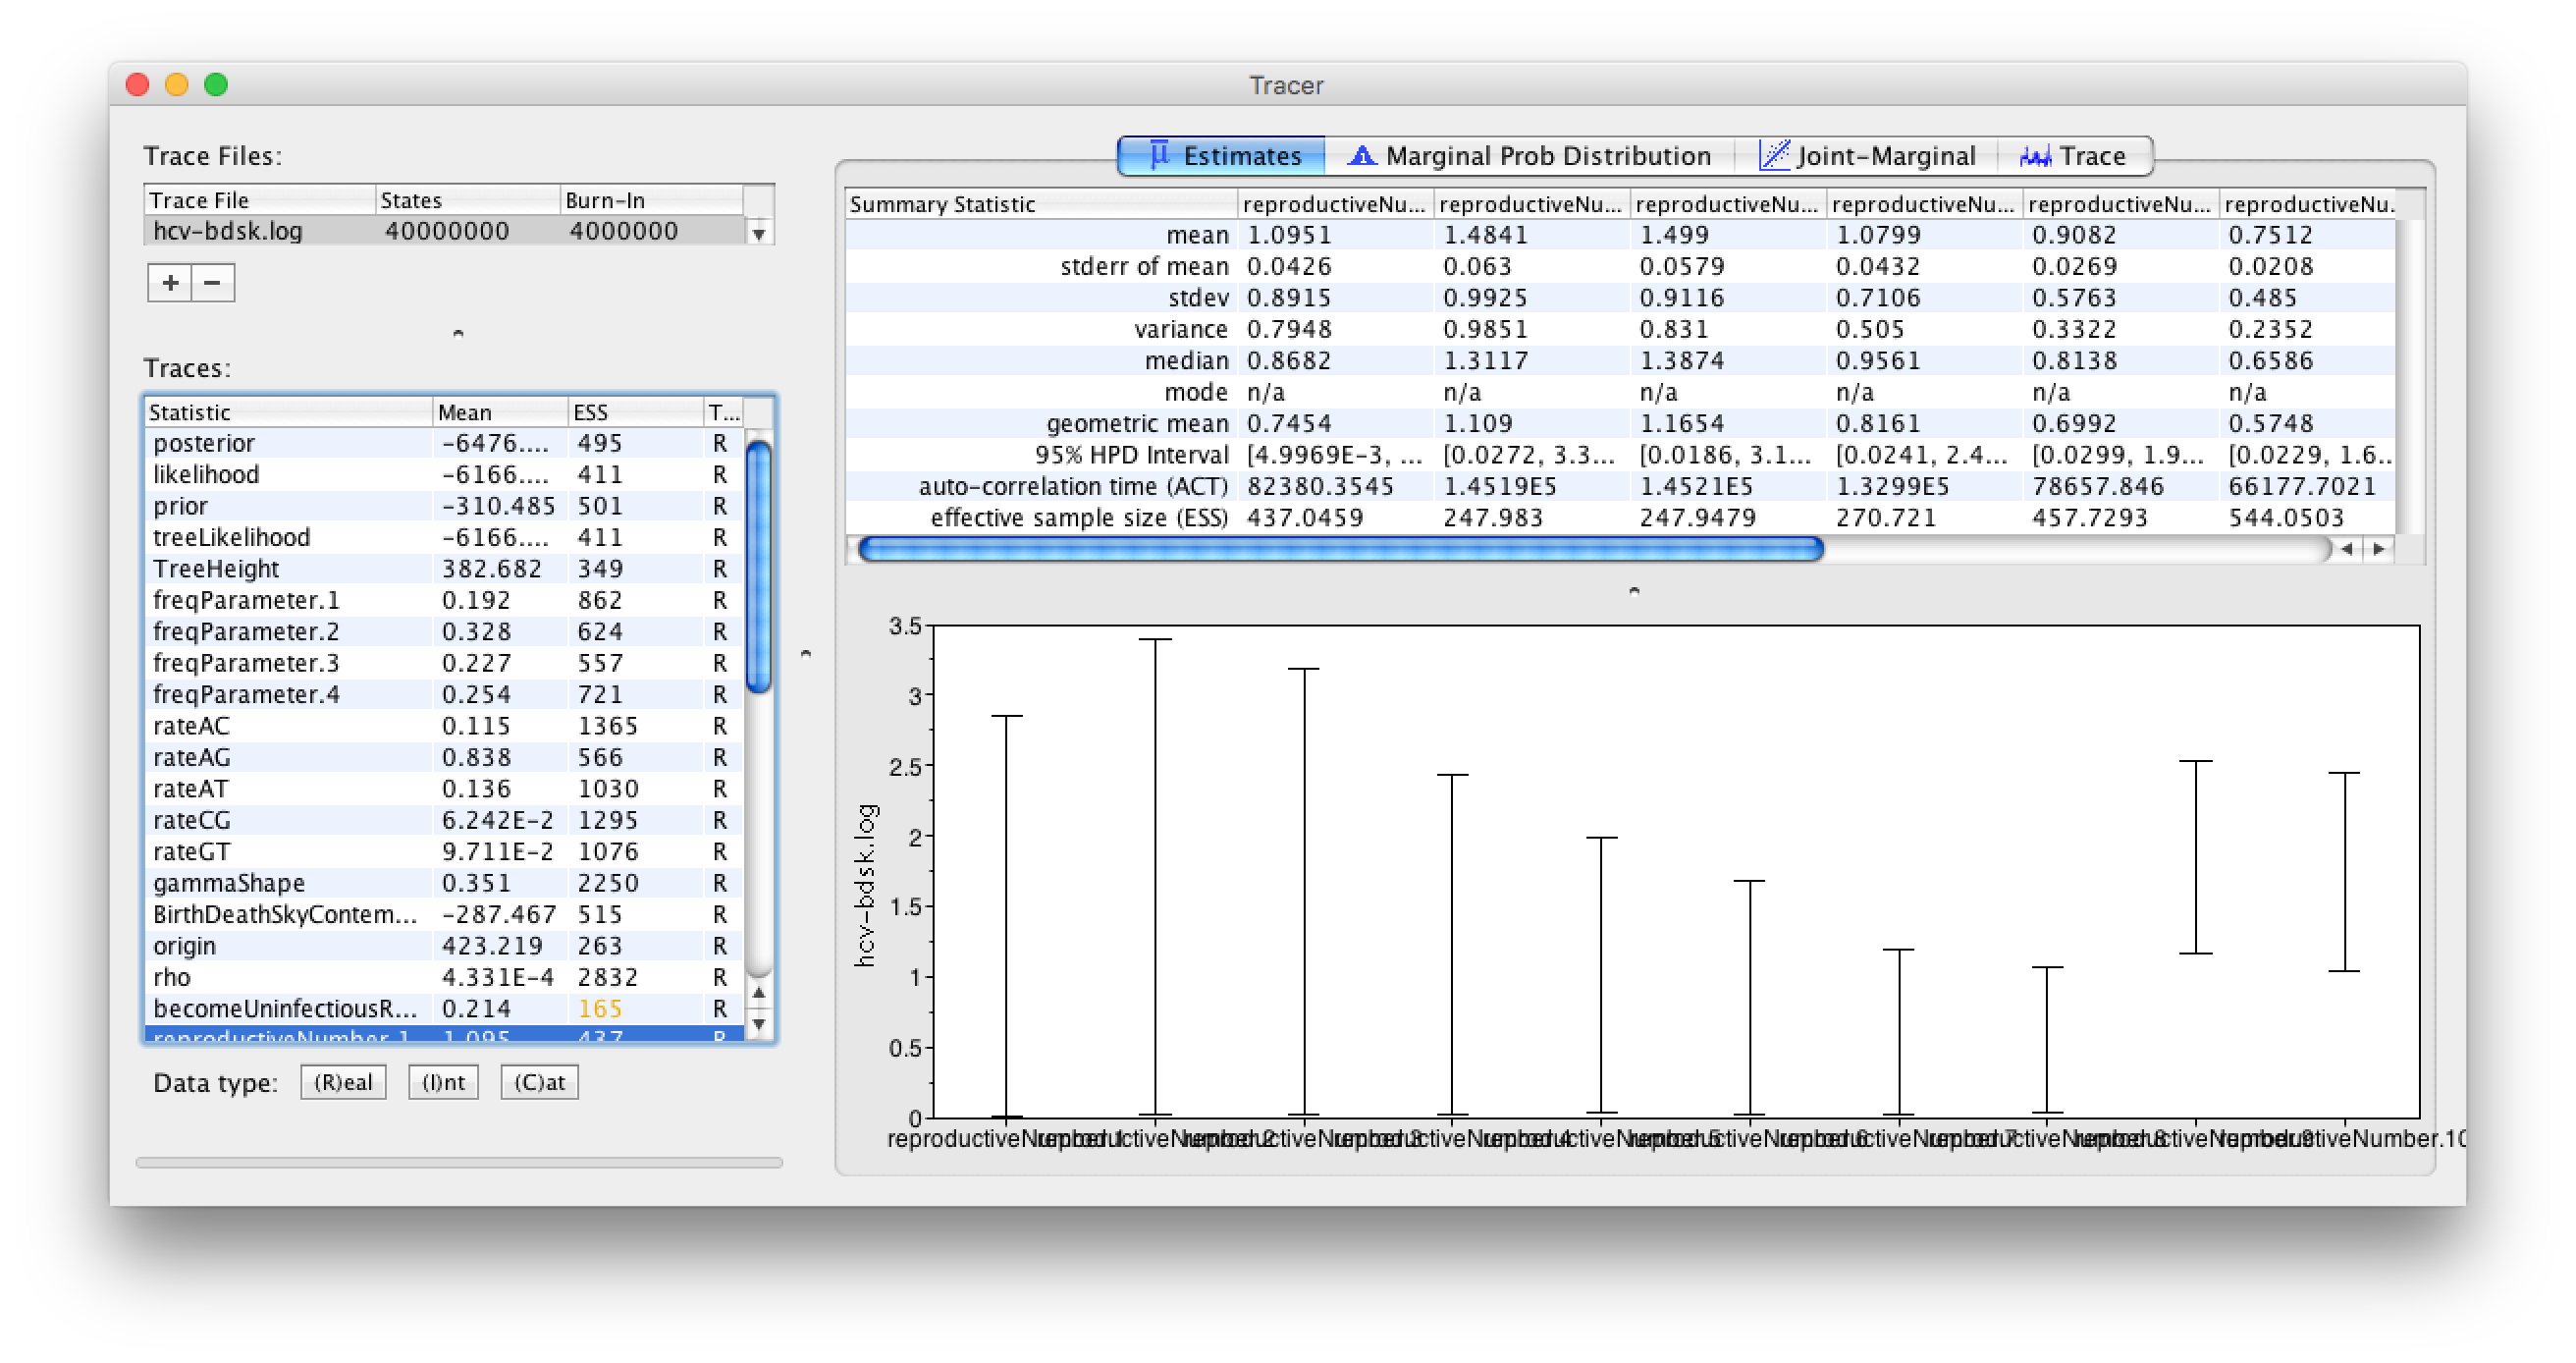
\includegraphics[width=\textwidth]{figures/bdsky_tracer.png}
\caption{\small Estimated population dynamics by BDSKY in Tracer.}
\label{fig:bdsky_dynamics}
\end{figure}


We will instead use some R scripts to plot the output of the bdsky. 
Open R and install two package using:
\begin{framed}
install.packages("boa");\\
install.packages("RColorBrewer");\\
\end{framed}

The first package is needed for statistical analyses of the run and the second one contains color schemes needed by the other R scripts. 
To plot the results, we need to describe in the file \texttt{Skyline$\_$Example.R} where our \texttt{*.log} file is (Figure~\ref{fig:r_script}).

\begin{figure}[h!]
\centering
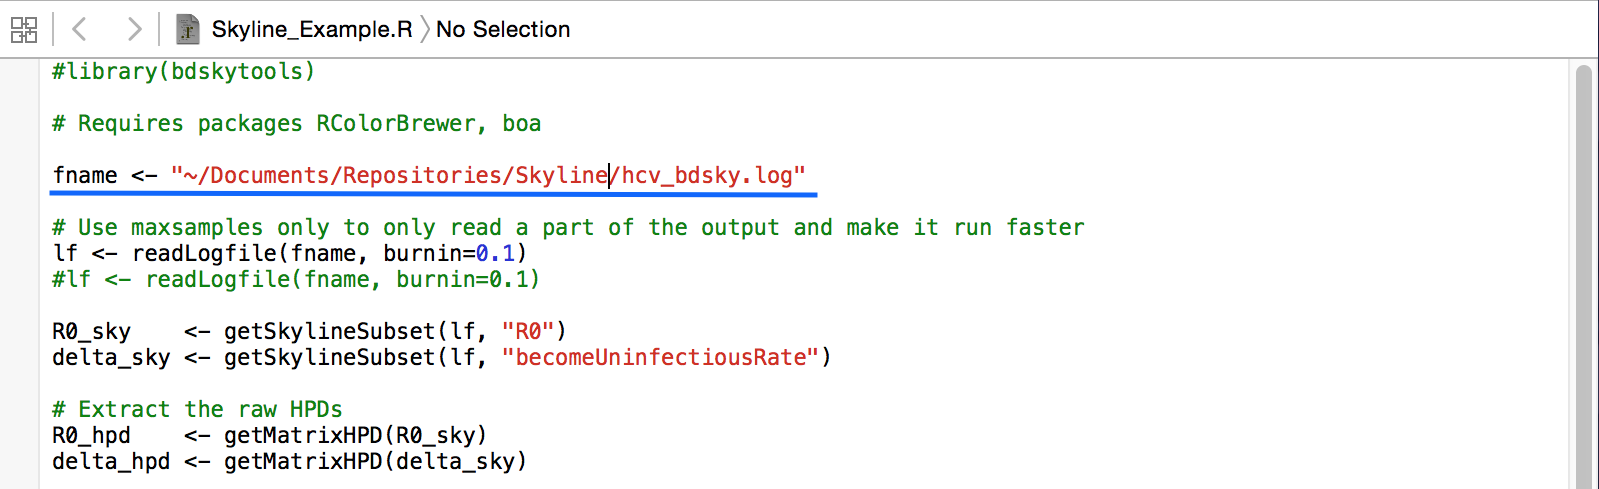
\includegraphics[width=\textwidth]{figures/find_log_file.png}
\caption{\small Put the path to the log file to fname in the R script.}
\label{fig:r_script}
\end{figure}

After saving the R script \texttt{Skyline$\_$Example.R}, we can now plot the analysis.
First, replace \texttt{dir} with the path to the directory where the R scripts are stored and then source the scripts. By default this is the \texttt{data} directory inside the tutorial. The first 3 R scripts contain functions for reading BEAST2 log files, extracting HPD intervals and plotting skylines\footnote{These files are part of an R package that will be available on CRAN in the nearby future. For the moment, if you are interested you are welcome to check out the development version at \url{http://github.com/laduplessis}  (Beta testers needed!)}.


\begin{framed}
source('/dir/Figure$\_$Utilities.R');\\
source('/dir/Logfile$\_$Utilities.R');\\
source('/dir/SkylinePlot.R');
\end{framed}

Now you can either step through the commands in \texttt{Skyline$\_$Example.R} one by one or source it as with the others. 

\begin{framed}
source('/dir/Skyline$\_$Example.R');
\end{framed}

First, the script loads the logfile and calculates the HPD intervals for $R_0$ and the becoming noninfectious rate. 

\begin{framed}
lf     <- readLogfile(fname, burnin=0.1) \\
R0\_sky <- getSkylineSubset(lf, \"R0\") \\
 \\
\# Extract the raw HPDs \\
R0\_hpd    <- getMatrixHPD(R0\_sky) \\
delta\_hpd <- getHPD(lf\$becomeUninfectiousRate) 
\end{framed}

Next we plot the raw HPD intervals of $R_0$. This is equivalent to the output in tracer. 

\begin{framed}
plotSkyline(1:10, R0\_hpd, type=\'step\')
\end{framed}

In order to plot the smooth skyline we have to calculate the HPD on a finer timegrid. To do this we first calculate the marginal posterior at every time of interest using the function \texttt{gridSkyline} and then calculate the HPD for each of the finer time intervals. 

\begin{framed}
timegrid <- seq(1,400,length.out=100) \\
R0\_gridded     <- gridSkyline(R0\_sky,    lf\$origin, timegrid) \\
R0\_gridded\_hpd <- getMatrixHPD(R0\_gridded)
\end{framed}

Now we are ready to plot the smooth skyline

\begin{framed}
\# The plotting times, the most recent sample is 1993 \\
times     <- 1993-timegrid \\
plotSkyline(times, R0\_gridded\_hpd, type='smooth')
\end{framed}


We can plot the gridded skyline (not its HPDs) for a few of the samples to see what it really looks like. Note that the intervals overlap between different posterior samples. This is because the origin is different in each sample. As we add more samples to the plot we start to see the smooth skyline appear. 

\begin{framed}
plotSkyline(times, R0\_gridded, type='steplines', traces=10, col=pal.dark(cblue,0.5),ylims=c(0,5)) \\
plotSkyline(times, R0\_gridded, type='steplines', traces=100, col=pal.dark(cblue,0.5),ylims=c(0,5)) \\
plotSkyline(times, R0\_gridded, type='steplines', traces=1000, col=pal.dark(cblue,0.1),ylims=c(0,5))
\end{framed}

Finally, we can plot both the $R_0$ and the becoming noninfectious rate on a single set of axes. Since we left the dimension of the becoming noninfectious rate at 1, it is constant through time. (Normally we would not plot constant parameters over a time period). The output should be similar to figure~\ref{fig:bdsky_out}

\begin{framed}
plotSkylinePretty(range(times), as.matrix(delta\_hpd), type='step', axispadding=0.0, col=pal.dark(cblue), fill=pal.dark(cblue, 0.5), col.axis=pal.dark(cblue), \\
ylab=expression(delta), side=4, yline=2, ylims=c(0,1), xaxis=FALSE) \\
plotSkylinePretty(times, R0\_gridded\_hpd, type='smooth', axispadding=0.0, col=pal.dark(corange), fill=pal.dark(corange, 0.5), col.axis=pal.dark(corange), \\
xlab="Time", ylab=expression(\"R\"[0]), side=2, yline=2.5, xline=2, xgrid=TRUE, ygrid=TRUE, gridcol=pal.dark(cgray), ylims=c(0,3), new=TRUE, add=TRUE) 
\end{framed}

\begin{figure}[h!]
\centering
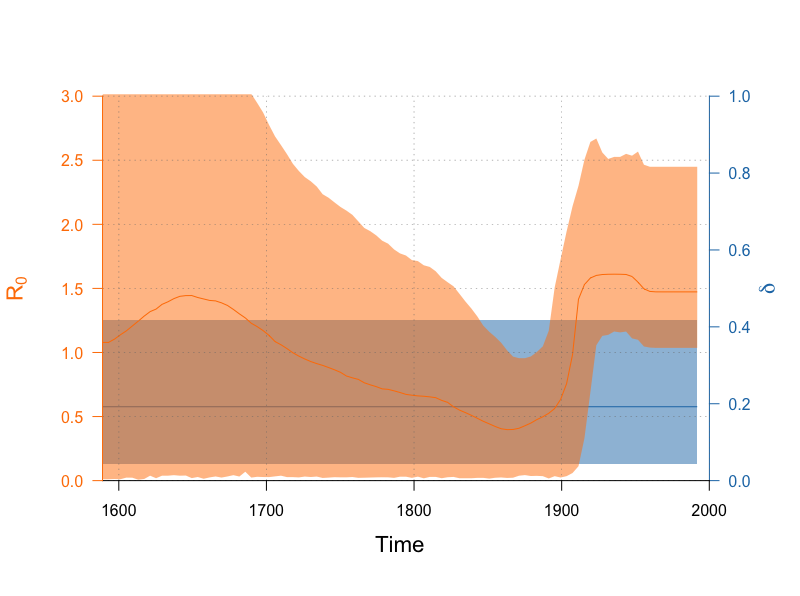
\includegraphics[width=0.5\textwidth]{figures/bdsky_output.png}
\caption{\small Estimates of the inferred R$_{0}$ (orange) over time and the estimate of the becoming un-infectious rate (blue), for which we only used one value .}
\label{fig:bdsky_out}
\end{figure}


\subsubsection{Some considerations for using the Skyline}

Both the coalescent and the birth-death skylines assume that the population is well-mixed. That is, they assume that there is no significant population structure and that the sequences are a random sample from the population. However, if there is population structure, for instance sequences were sampled from two different villages and there is much more contact within than between villages, then the results will be biased~\citep{Heller2013}. Instead a structured model should be used to account for these biases.


%%%%%
\bigskip
\section{Useful Links}

\begin{itemize}
\item \href{http://www.beast2.org/book.html}{\textit{Bayesian Evolutionary Analysis with BEAST 2}}  \citep{BEAST2book2014}
\item BEAST 2 website and documentation: \href{http://www.beast2.org/}{http://www.beast2.org/} 
\item BEAST 1 website and documentation: \href{http://beast.bio.ed.ac.uk}{http://beast.bio.ed.ac.uk}
\item Join the BEAST user discussion: \href{http://groups.google.com/group/beast-users}{http://groups.google.com/group/beast-users} 
\end{itemize}

%Questions about this tutorial can be directed to Tracy Heath (email: \href{mailto:tracyh@berkeley.edu}{tracyh@berkeley.edu}).

\href{http://creativecommons.org/licenses/by/4.0/}{\includegraphics[scale=0.8]{figures/ccby.pdf}} This tutorial was written by \href{https://www.bsse.ethz.ch/cevo/the-group/people/person-detail.html?persid=181412}{Nicola M\"{u}ller} for the \href{https://www.bsse.ethz.ch/cevo/taming-the-beast.html}{Taming the BEAST Workshop} on applied phylogenetics and molecular evolution and is licensed under a \href{http://creativecommons.org/licenses/by/4.0/}{Creative Commons Attribution 4.0 International License}. 



Version dated: \today



\newpage

%%%%%%%%%%%%%%%%%%%%%%%%%%%%%%%%%%%%
%  REFERENCES  
%%%%%%%%%%%%%%%%%%%%%%%%%%%%%%%%%%%%

\printbibliography[heading=relevref]



\end{document}
